\documentclass[a4paper]{article}
\linespread{1.6}
\usepackage{enumerate}
\usepackage{geometry}
\usepackage{setspace}
\usepackage{amsmath}
\usepackage{amssymb}
\usepackage{cite}
\usepackage[pdftex]{graphicx}
\usepackage{float}
\usepackage{subfigure}
\usepackage{listings}
\geometry{left=1.4cm,right=1.4cm,top=2.5cm,bottom=2.5cm}

\begin{document}
\begin{spacing}{2.0}
\begin{flushleft}\begin{huge}EEL5840 Fundamental Machine Learning   Homework 4\end{huge}\end{flushleft}
\begin{flushright}\begin{Large} Hudanyun Sheng \end{Large}\end{flushright}

%\Large{All the code used are attached at the end of this report.}


\paragraph{\huge\textbf{ Question 1\\} }
\normalsize
It is attached in the separate file.
\paragraph{\huge\textbf{ Question 2\\} }
\normalsize
It is attached in the separate file.

\paragraph{\huge\textbf{ Question 3\\} }
\normalsize
\noindent
The code is attached at the end of this file.\\
Suppose the true mean of the Gaussian distribution is 2 ($\mu = 2$). And we are drawing random samples from this Gaussian distribution, with a Gaussian prior distribution on the mean parameters. Assume the variance for the Gaussian likelihood and Gaussian prior is fixed and known. And our goal is to estimate the mean. Since we are to explore how do the initial values of the prior mean, prior variance and likelihood variance interact to effect the final estimate of mean, below shows my experiment design, for each experiment I draw 10 samples. 
\begin{table}[htbp]
\centering
\begin{tabular}{lccc}
\hline
{ } & $\mu_0$ & $\sigma_0$ & $\sigma$ \\ \hline
{ 1} & $4$ & $0.5$ & $0.5$ \\
{ 2} & { } & $0.5$ & $5$ \\
{ 3} & { } & $5$ & $0.5$ \\ 
{ 4} & { } & $5$ & $5$ \\\hline
{ 5} & $2$ & $0.5$ & $0.5$ \\
{ 6} & { } & $0.5$ & $5$ \\
{ 7} & { } & $5$ & $0.5$ \\ 
{ 8} & { } & $5$ & $5$ \\\hline
\end{tabular}
\caption{Experiment design}
\end{table}
As stated in the instruction, at the very beginning we have some initial assumption of the prior distribution, i.e. $p(\mu|\mu_0) = N(\mu|\mu_0, \sigma_0^2)$, and with every sample drawn from the true distribution, the maximum likely estimate of mean is calculated as the sample, i.e. $\mu_{ML} = \bar x$, the maximum a posterior estimate of mean is also calculated using $\mu_N = \displaystyle\frac{\sigma^2}{N\sigma_0^2 + \sigma^2}\mu_0 + \displaystyle\frac{N\sigma_0^2}{N\sigma_0^2 + \sigma^2}\mu_{ML}$. And then this MAP solution of mean is used as the prior information, and used in calculation with the coming sample drawn. \\
The results of the experiments described above are attached in next several pages.

\newpage
The table of experiment results from first 10 draws from Gaussian:
\begin{figure}[H]
\centering
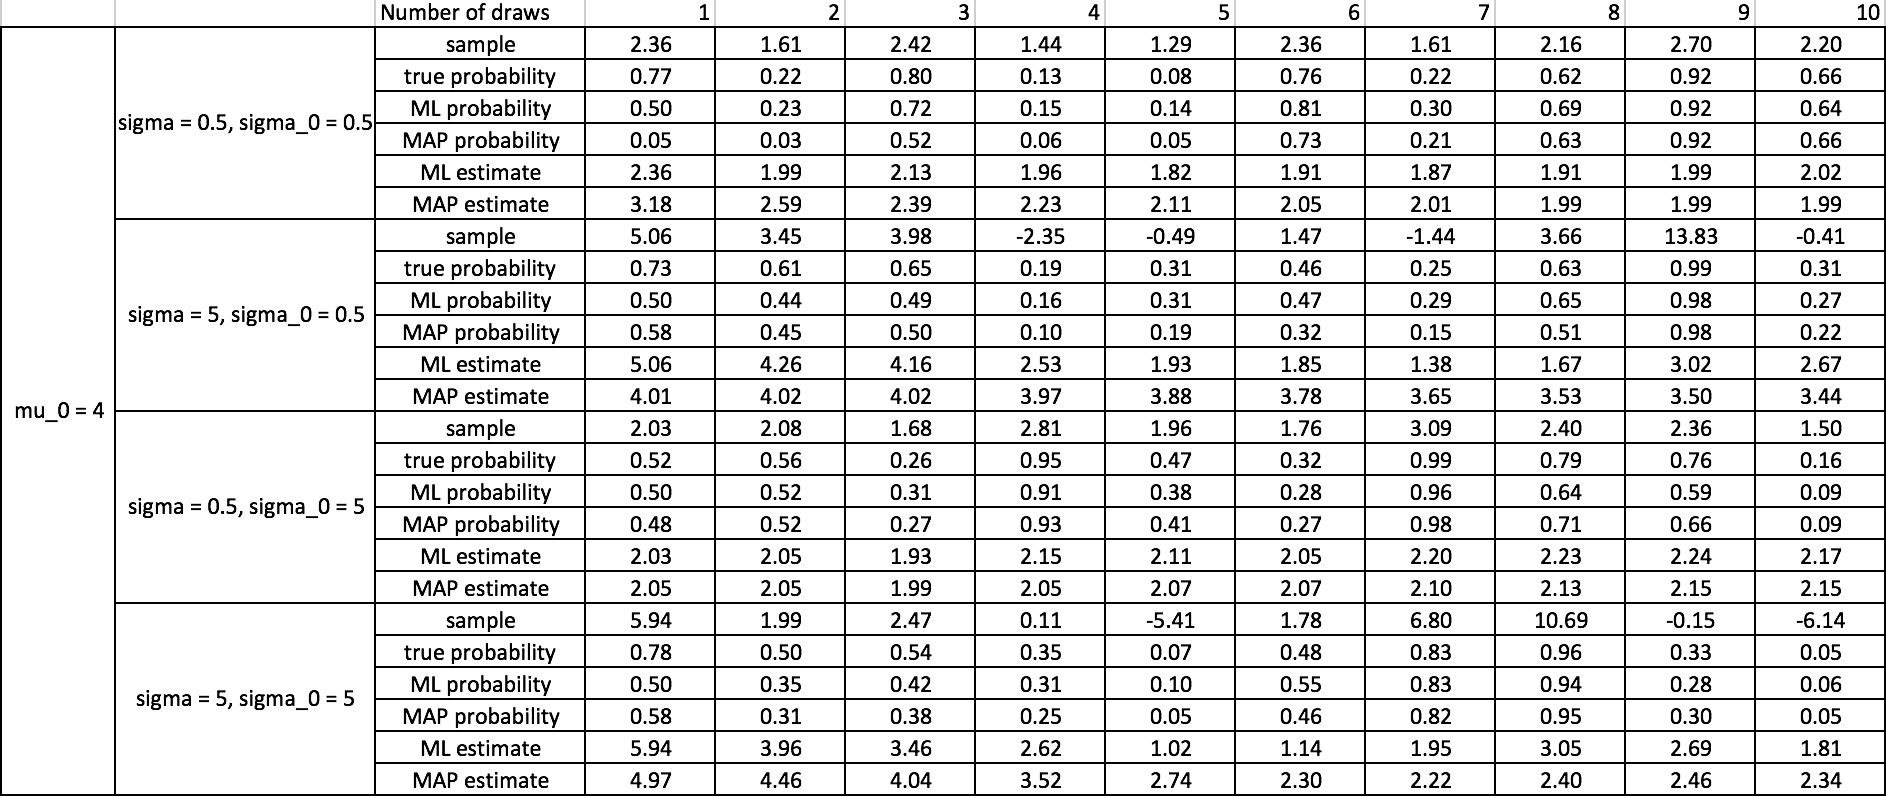
\includegraphics[width = 7.5in]{exp1.jpg}
\caption{Experimental Results with ``wrong" prior}
\label{fig1}
\end{figure}

\begin{figure}[H]
\centering
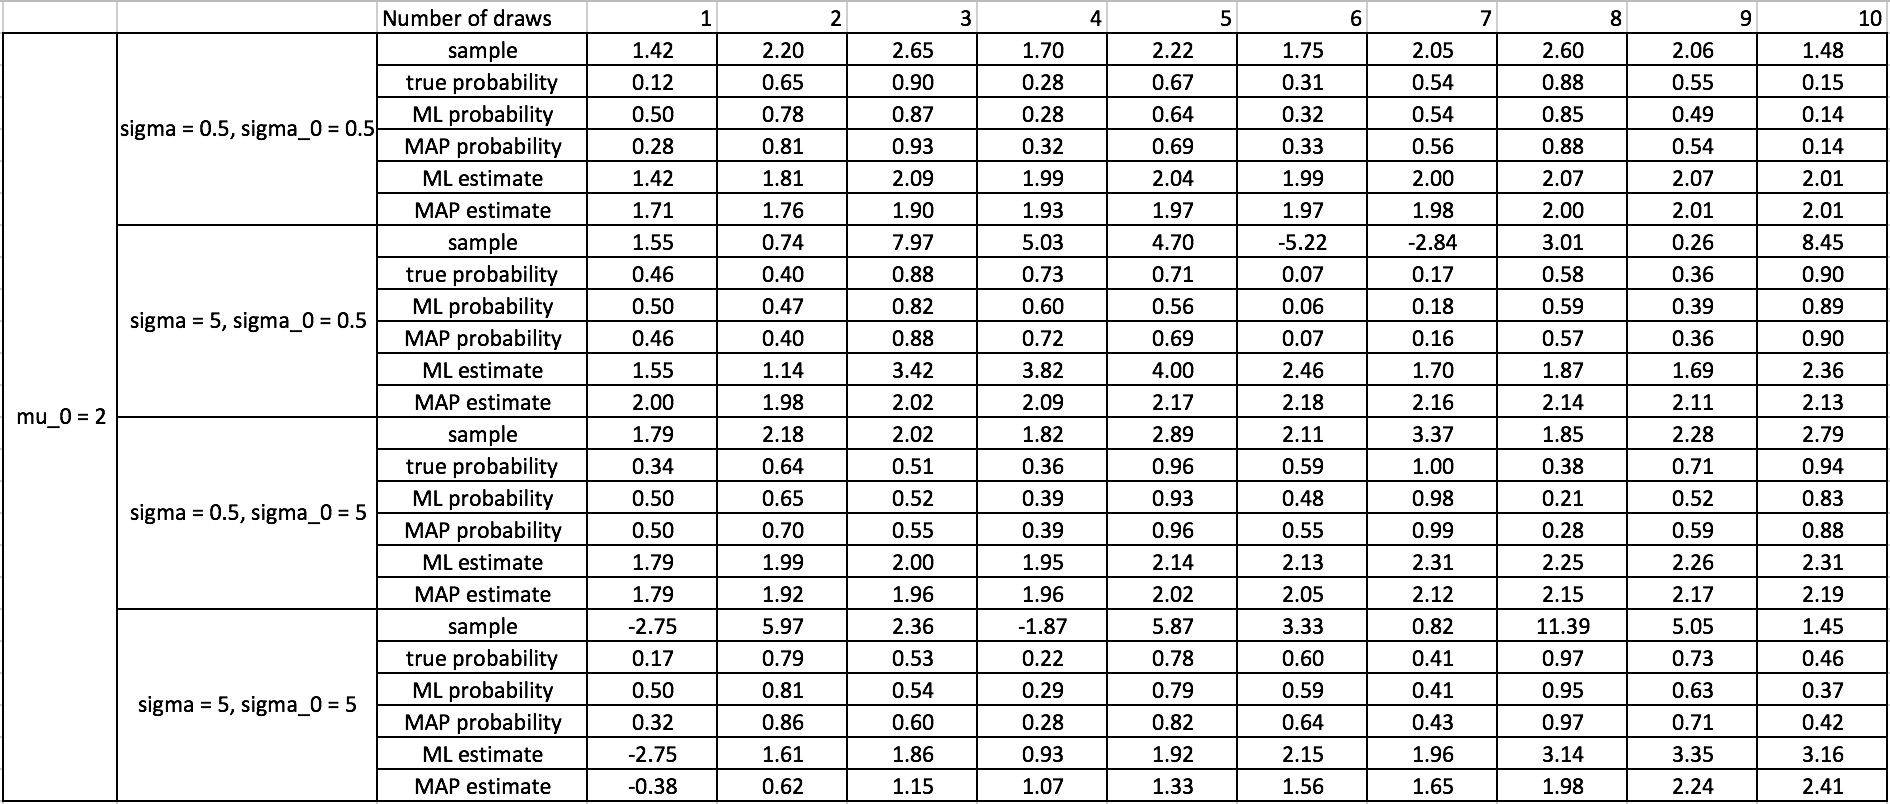
\includegraphics[width = 7.5in]{exp2.jpg}
\caption{Experimental Results with ``right" prior}
\label{fig1}
\end{figure}

We can see from the experiment result that when more samples are drawn, both the ML probability and the MAP probability are approaching the true probability, and at the same time, the both the ML estimate and the MAP estimate are also approaching the true mean, or tend to approach, no matter how initialized. 
The corresponding figures and analysis details are shown in the coming pages.
\begin{itemize}
\newpage
\item
Comparison of results when \textbf{prior mean} is initialized to be ``wrong" or ``right", with $\sigma = \sigma_0 = 0.5$ fixed.
\begin{figure}[H]
	\centering
	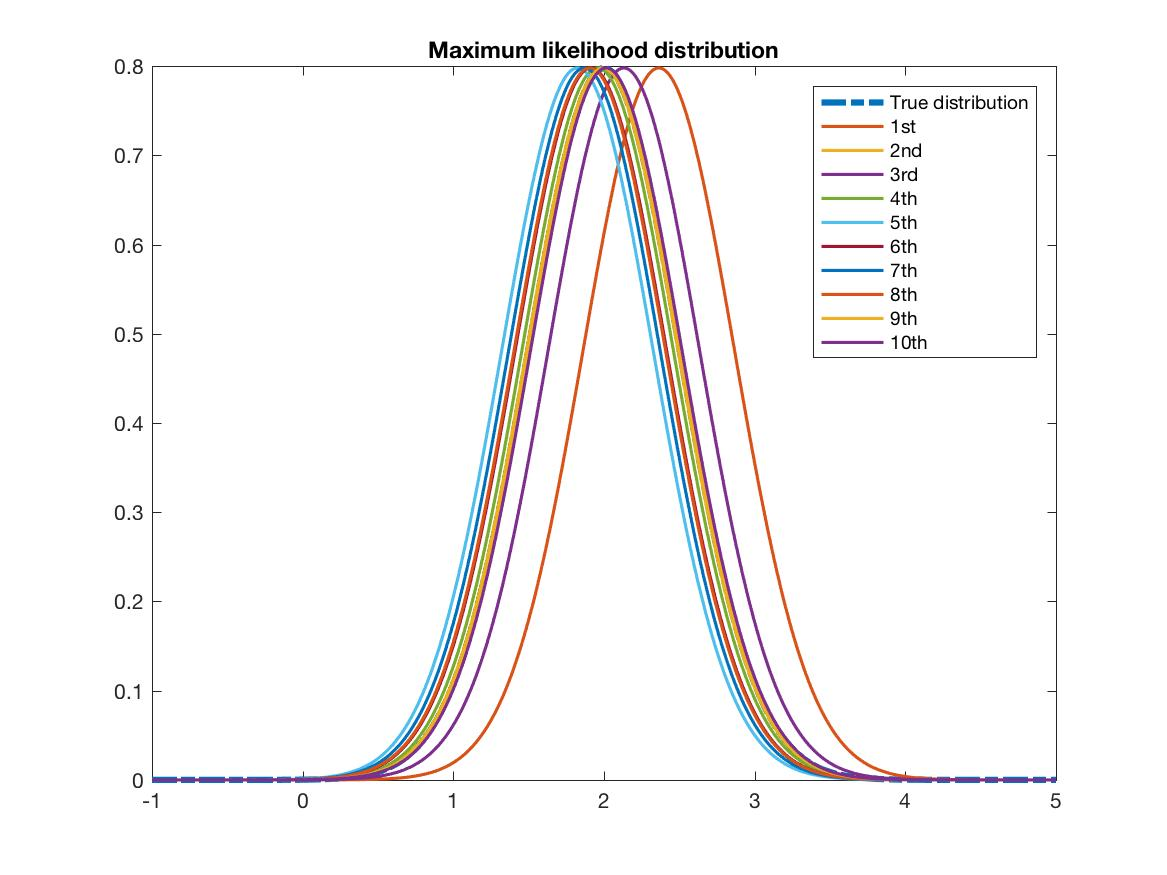
\includegraphics[width=3in]{ML1.jpg}
	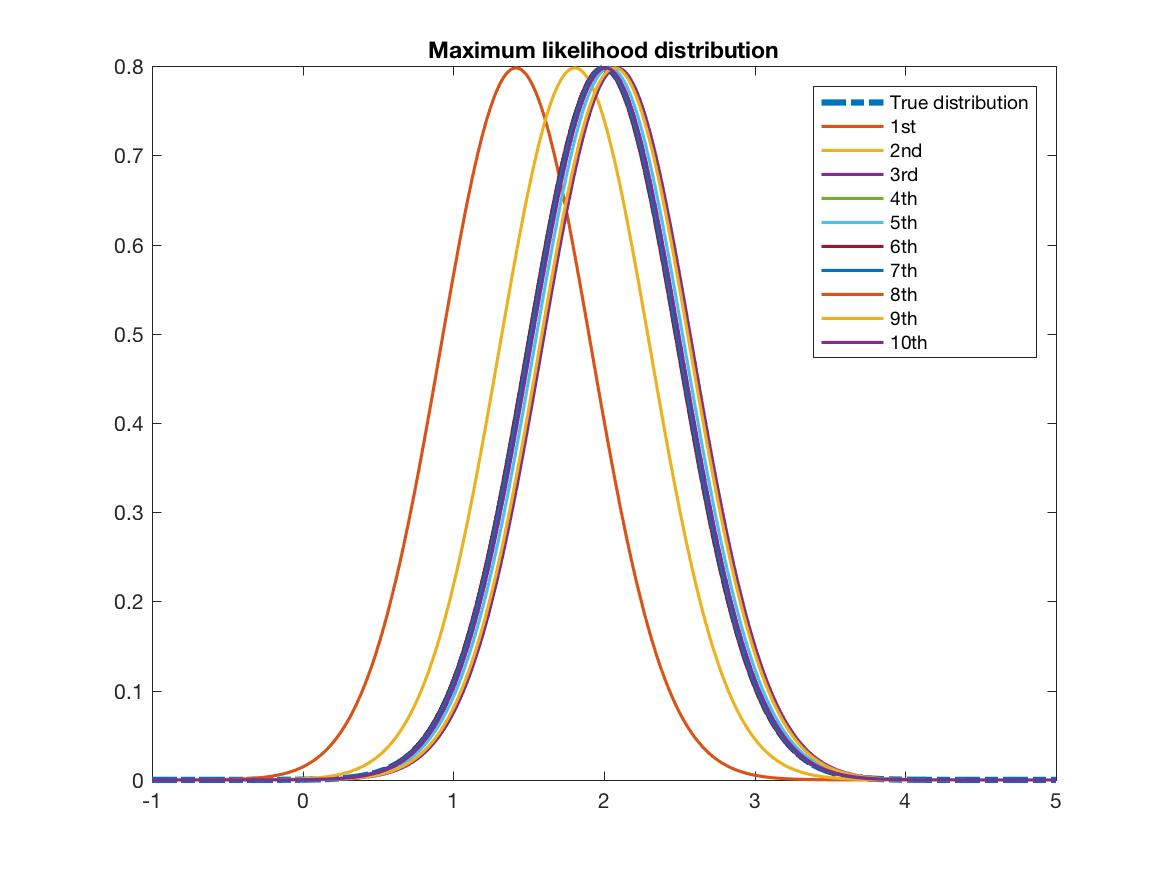
\includegraphics[width=3in]{ML5.jpg}
	\caption{left: ML with ``wrong" prior mean(Exp1). right: ML with ``right" prior mean(Exp5).}
	\label{q}
\end{figure}
\begin{figure}[H]
	\centering
	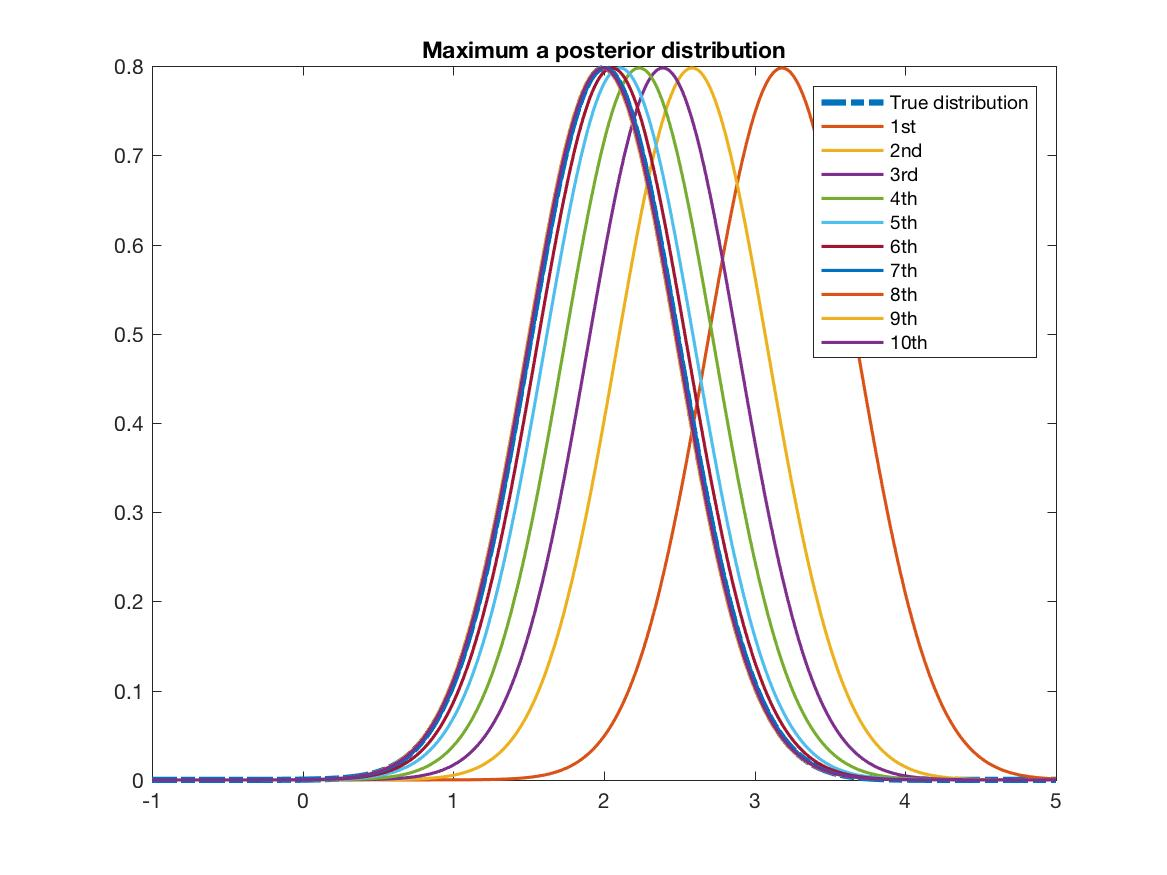
\includegraphics[width=3in]{MAP1.jpg}
	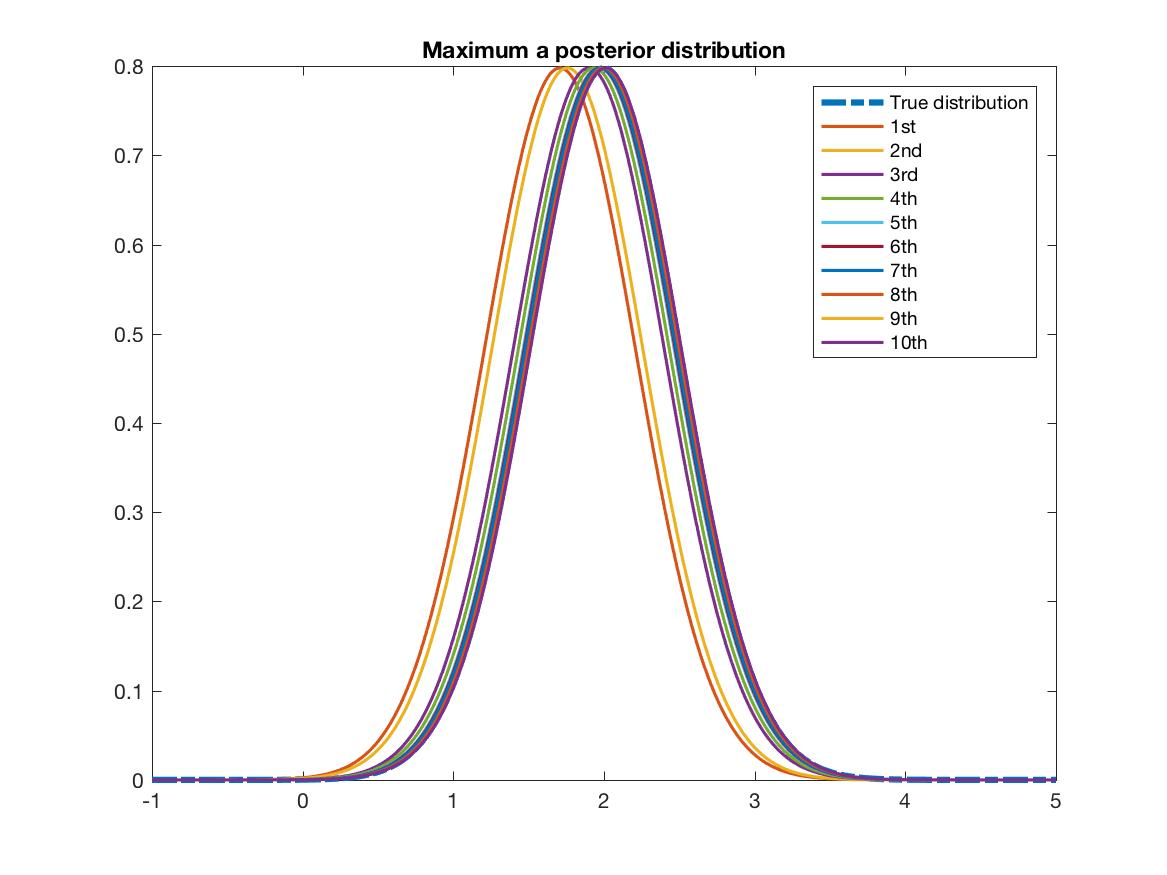
\includegraphics[width=3in]{MAP5.jpg}
	\caption{left: MAP with ``wrong" prior mean(Exp1). right: MAP with ``right" prior mean(Exp5).}
	\label{fig:side:b}
\end{figure}
\begin{figure}[H]
	\centering
	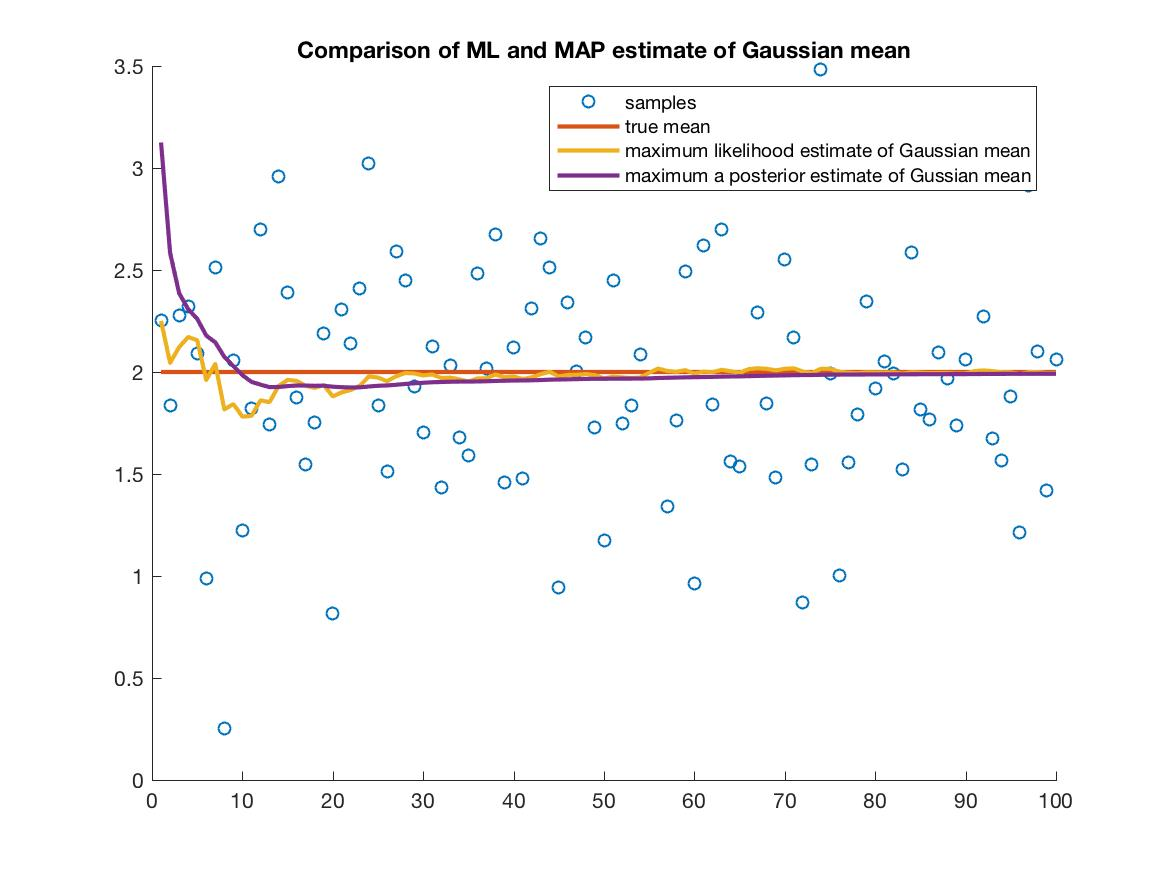
\includegraphics[width=3in]{100comparison1.jpg}
	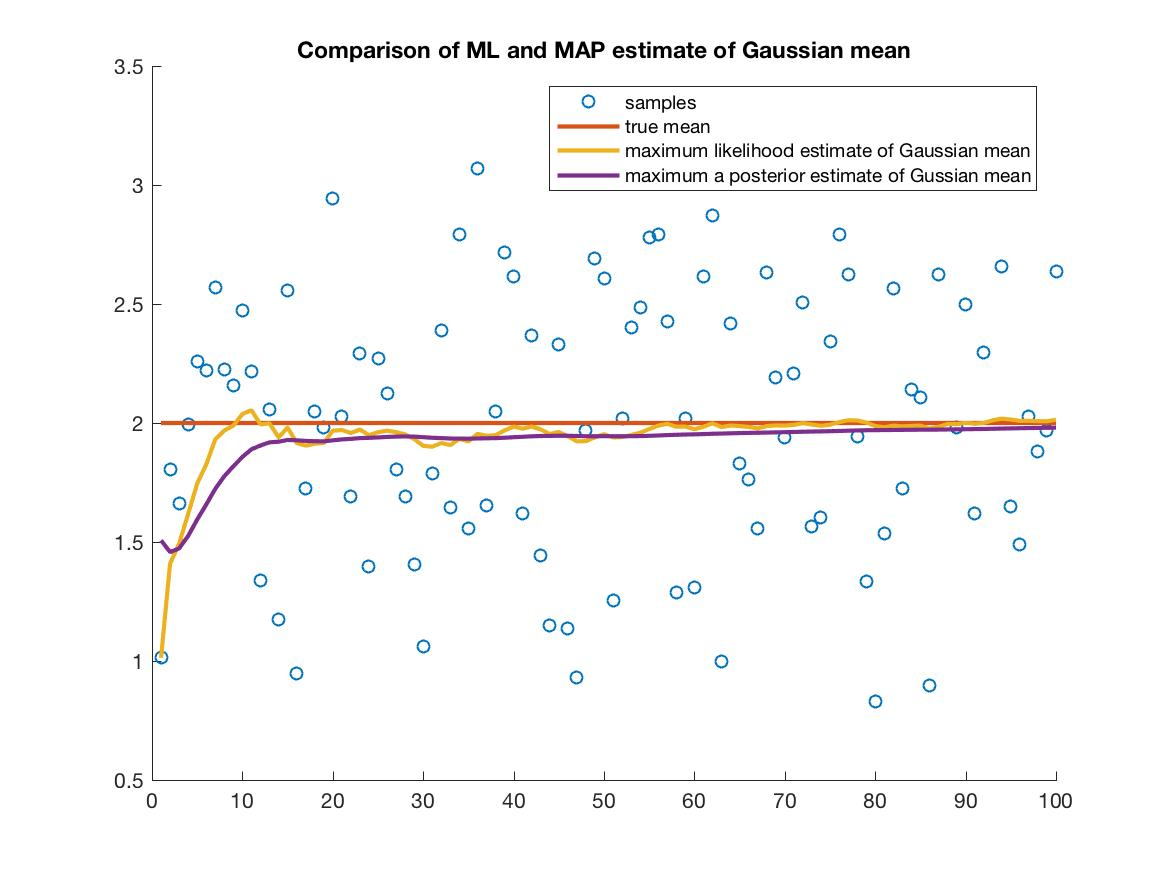
\includegraphics[width=3in]{100comparison5.jpg}
	\caption{left: comparison with ``wrong" prior mean(Exp1). right: comparison with ``right" prior mean(Exp5).}
	\label{fig:side:b}
\end{figure}
Compare the result with experiment 1 and experiment 5 (or equivalently 2 and 6, 3 and 7, 4 and 8), when the variance for the true distribution and the prior are fixed, and the prior mean is initialized to be ``wrong" or ``right", we can see that finally by both approach the distribution from ML and MAP would be very much similar to the true distribution. When the prior of the Gaussian is initialized to be a ``wrong" value, at first the MAP distribution is very different from the true distribution, because of the ``wrong" initial information, while if the prior of the Gaussian is initialized to be a ``right" value, the MAP distribution at first time would seem similar to the true distribution. Since the ML solution based solely on the data, the initialization of the prior mean will not affect the ML distribution. The difference shown in figure are only because of the randomness of sampling.\\

At the same time we compare the experiment results with larger variance on the prior (experiment 3 and 7), this pair of experiment are ones with larger prior variance compared to the former set.
\begin{figure}[H]
	\centering
	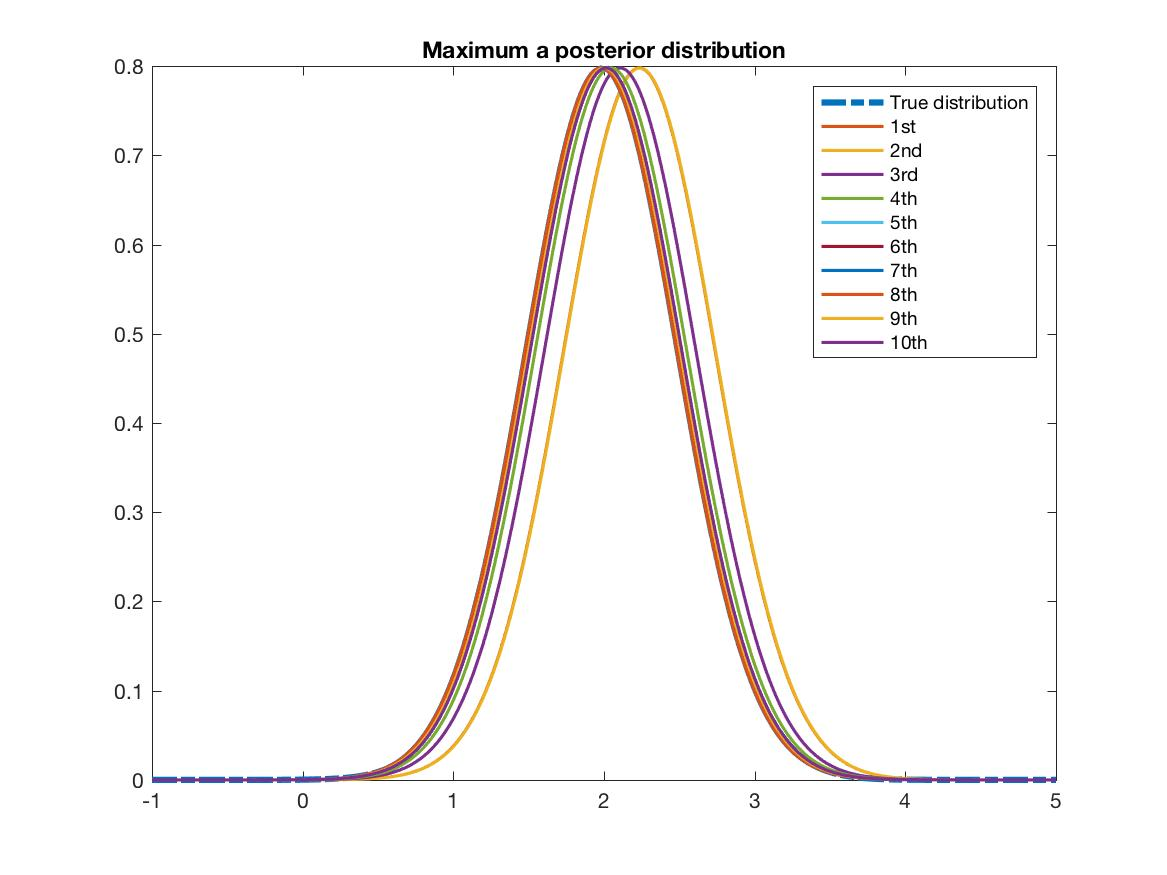
\includegraphics[width=3in]{MAP3.jpg}
	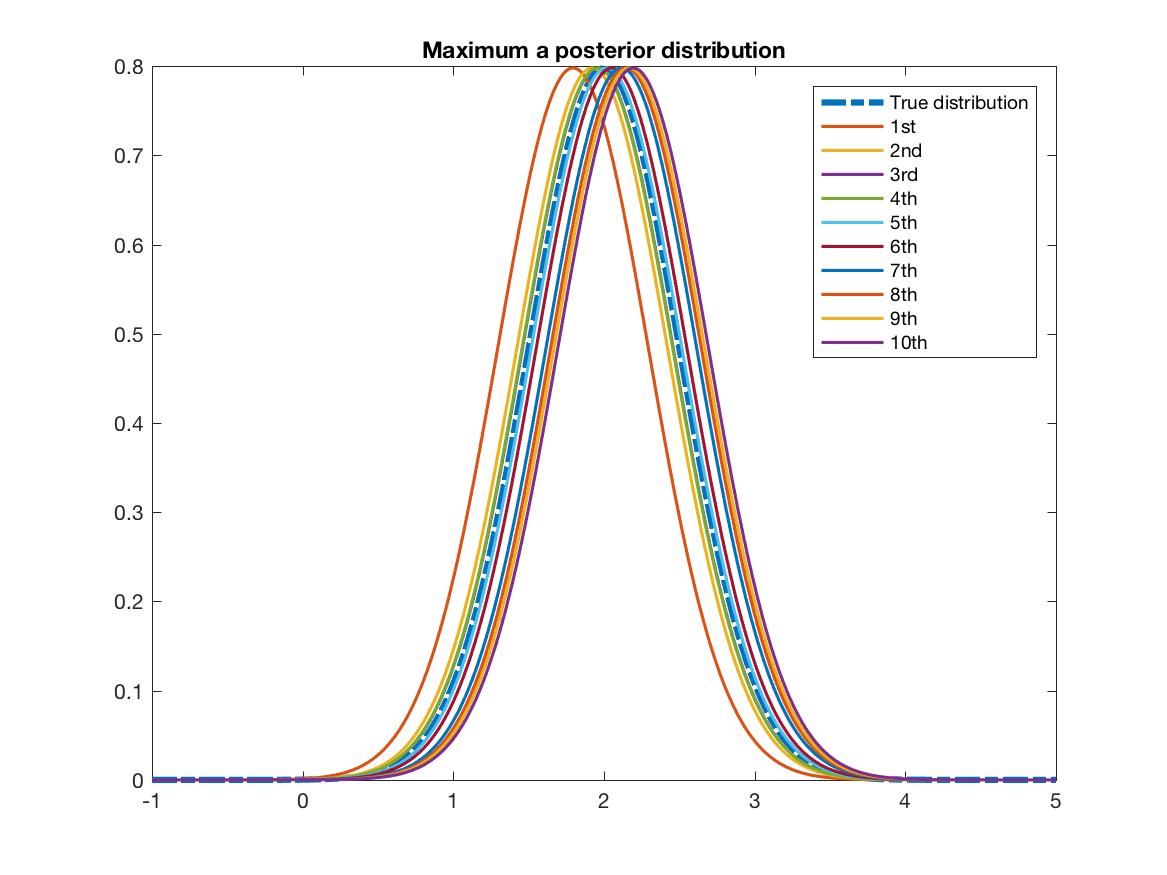
\includegraphics[width=3in]{MAP7.jpg}
	\caption{left: comparison with ``wrong" prior mean(Exp3). right: comparison with ``right" prior mean(Exp7).}
	\label{fig:side:b}
\end{figure}
Compare the results with these 2 groups of comparison, we can learn that when the variance of the prior is small, it is essential to choose a right value of the prior mean to get a better result of MAP; while when the  variance of the prior is large, the choose of prior mean is not that essential.

\newpage
\item
Comparison of varying \textbf{prior variance} from small to large by comparing the results of experiments 5 and 7, with $\mu_0 = 2$, $\sigma= 0.5$ fixed, $\sigma_0 = 0.5$(left) or $\sigma_0 = 5$(right).
\begin{figure}[H]
	\centering
	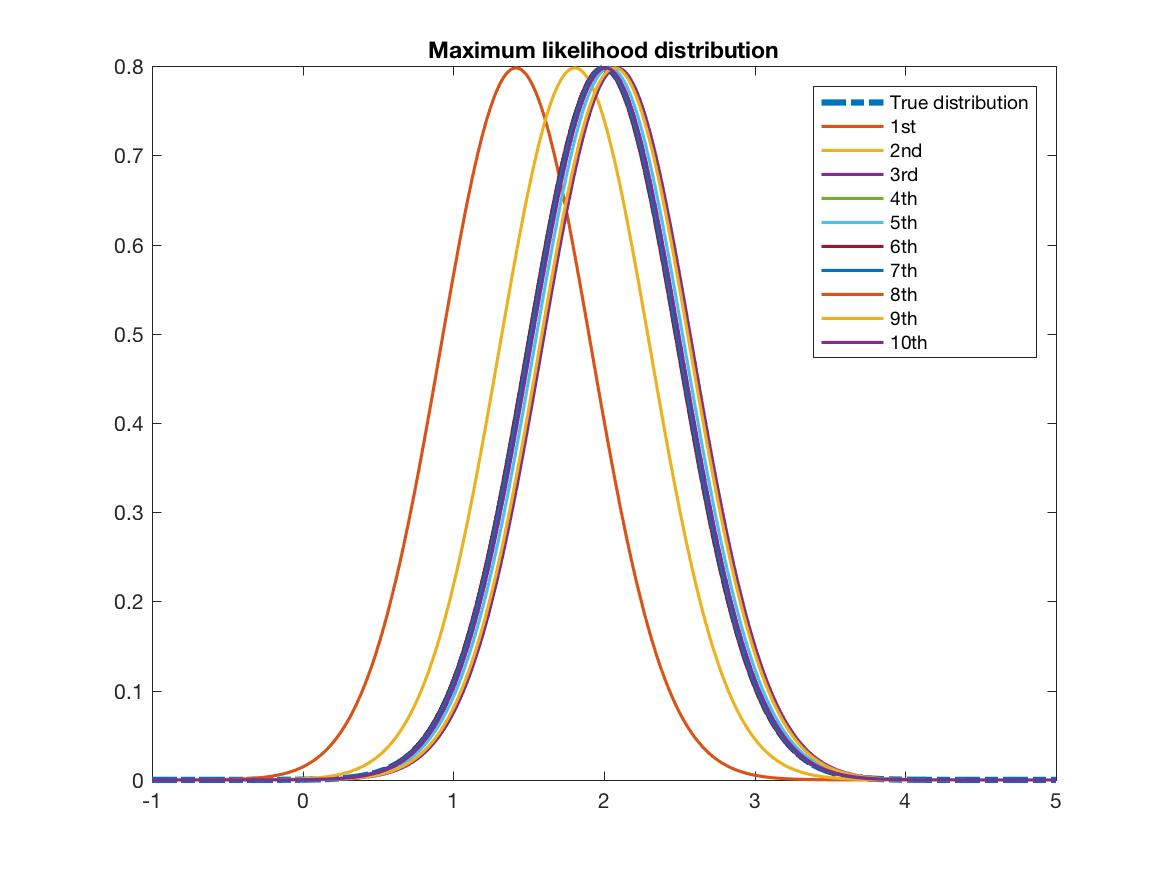
\includegraphics[width=3in]{ML5.jpg}
	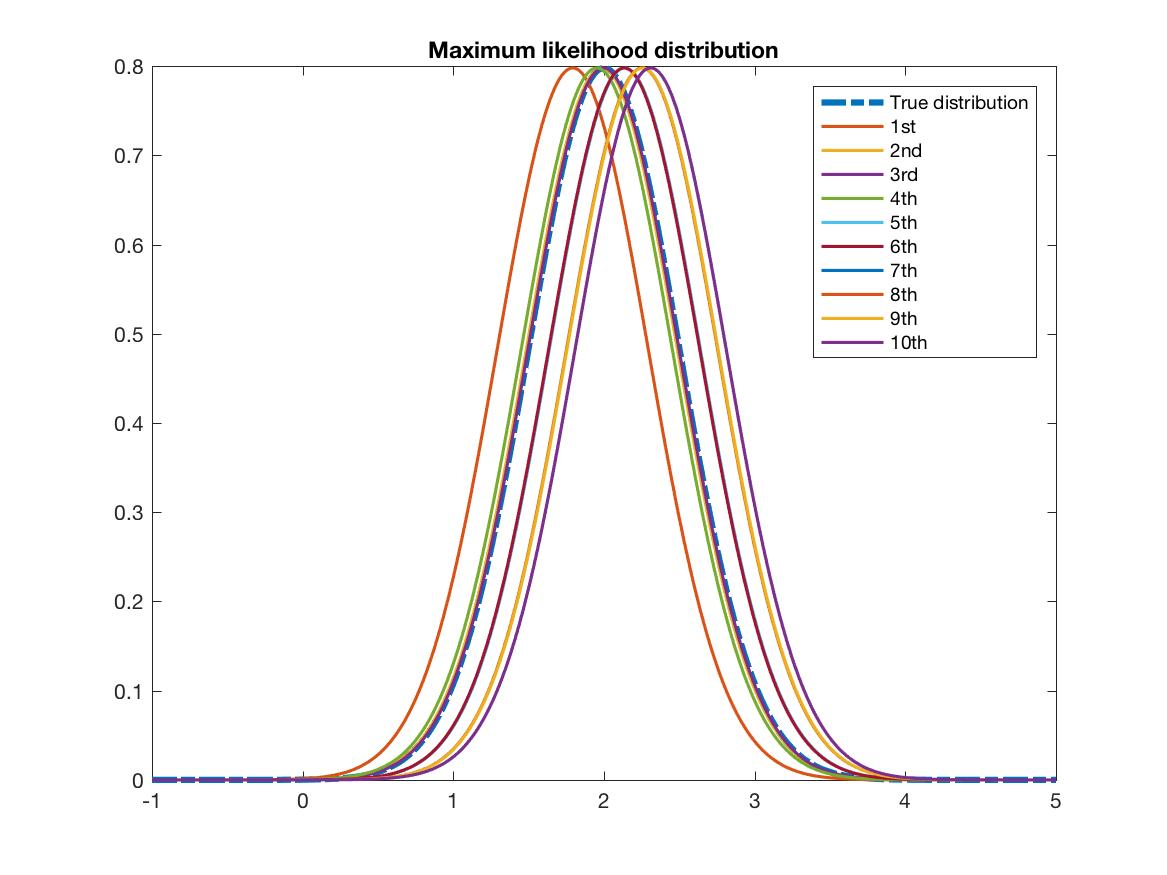
\includegraphics[width=3in]{ML7.jpg}
	\caption{left: ML with small prior variance(Exp5). right: ML with large prior variance(Exp7).}
	\label{q}
\end{figure}
\begin{figure}[H]
	\centering
	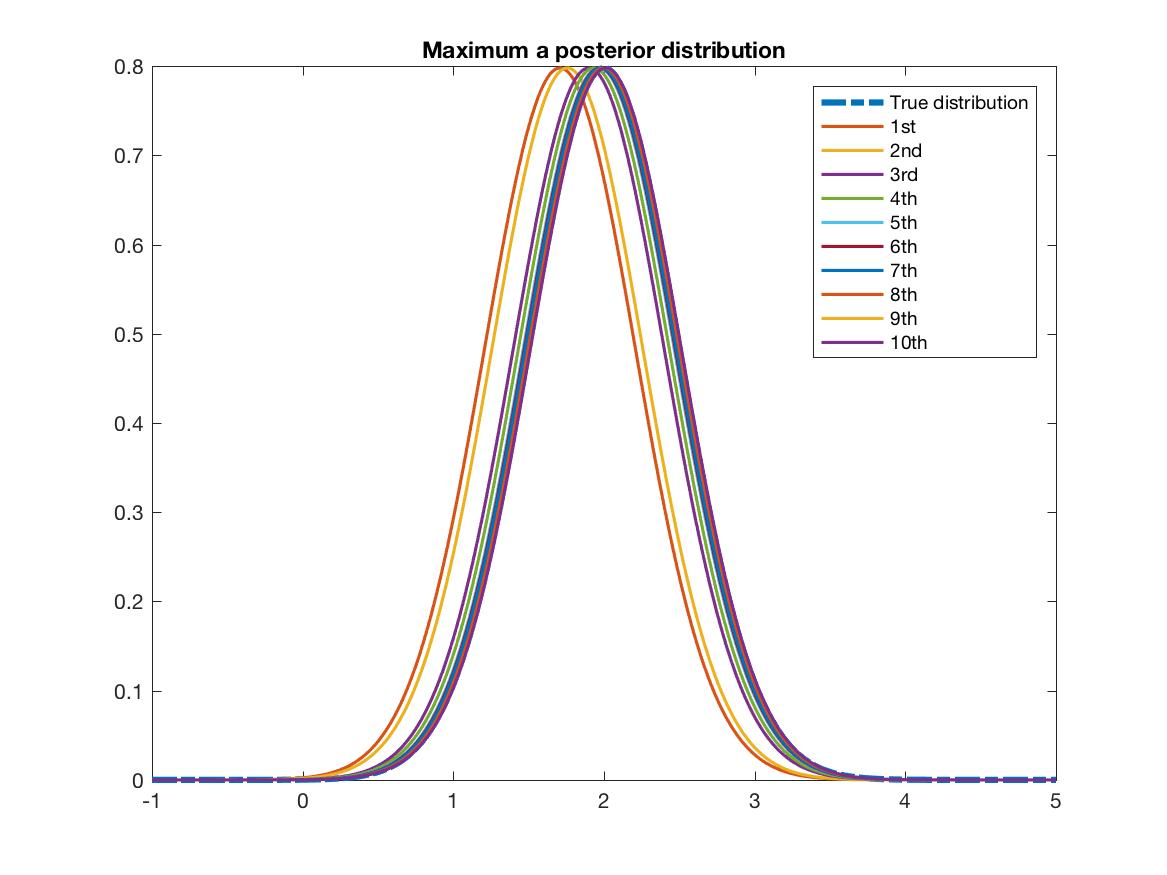
\includegraphics[width=3in]{MAP5.jpg}
	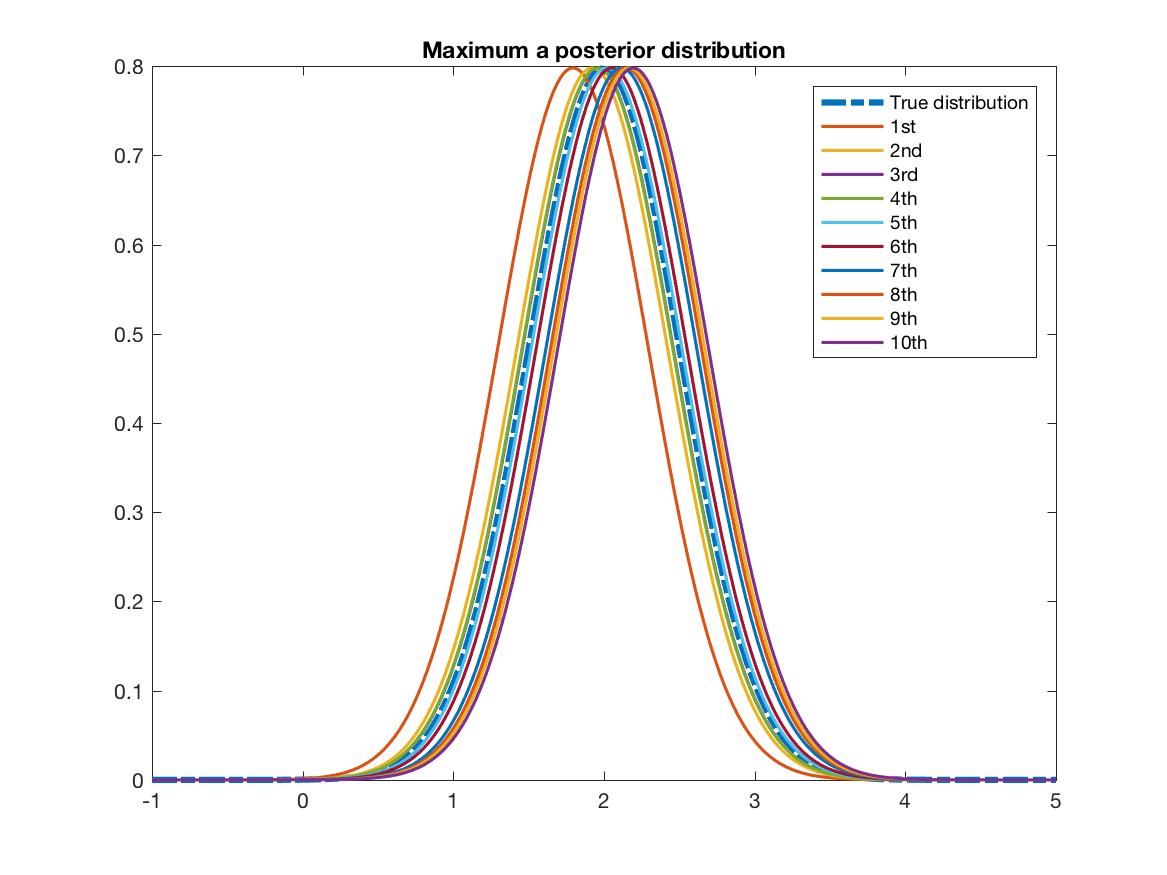
\includegraphics[width=3in]{MAP7.jpg}
	\caption{left: MAP with small prior variance(Exp5). right: MAP with large prior variance(Exp7).}
	\label{fig:side:b}
\end{figure}
\begin{figure}[H]
	\centering
	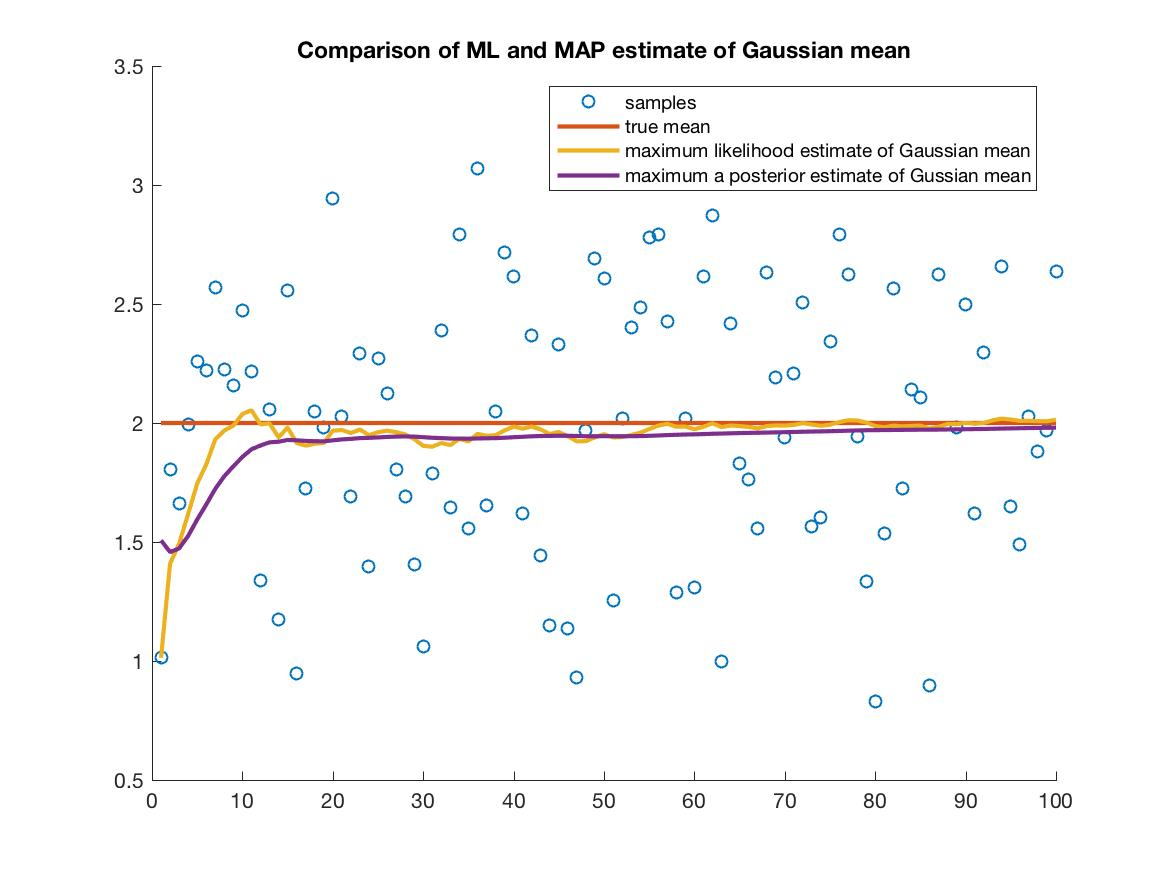
\includegraphics[width=3in]{100comparison5.jpg}
	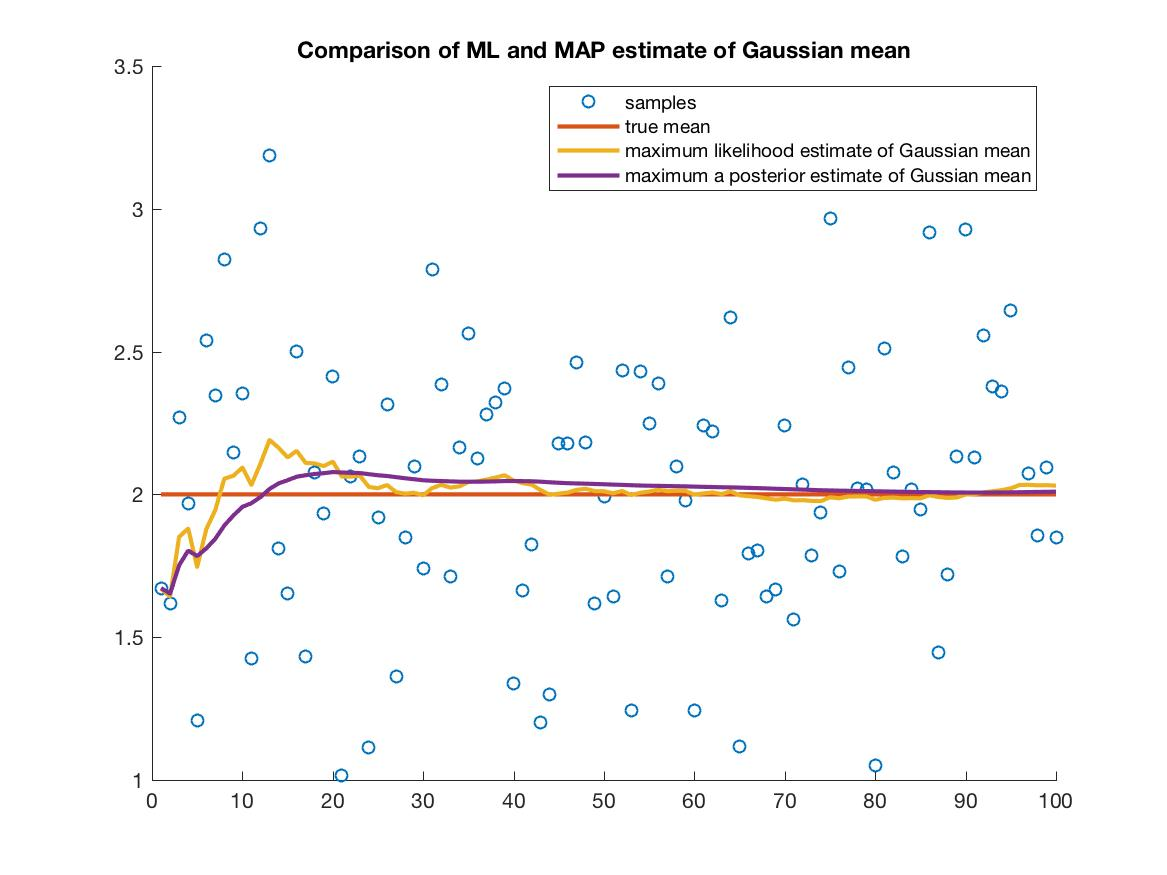
\includegraphics[width=3in]{100comparison7.jpg}
	\caption{left: comparison with small prior varianc(Exp5). right: comparison with arge prior variance(Exp7).}
	\label{fig:side:b}
\end{figure}
In this set of comparison I set the prior of mean to be the ``right" value, i.e. $\mu_0 = 2$. We have already known that the likelihood distribution based solely on the data, thus the changing of $\sigma_0$ would affect only the MAP result. When enough sample been drawn, both the $\mu_{ML}$ and $\mu_{MAP}$ would converge to the true mean of the distribution. 
\begin{figure}[H]
	\centering
	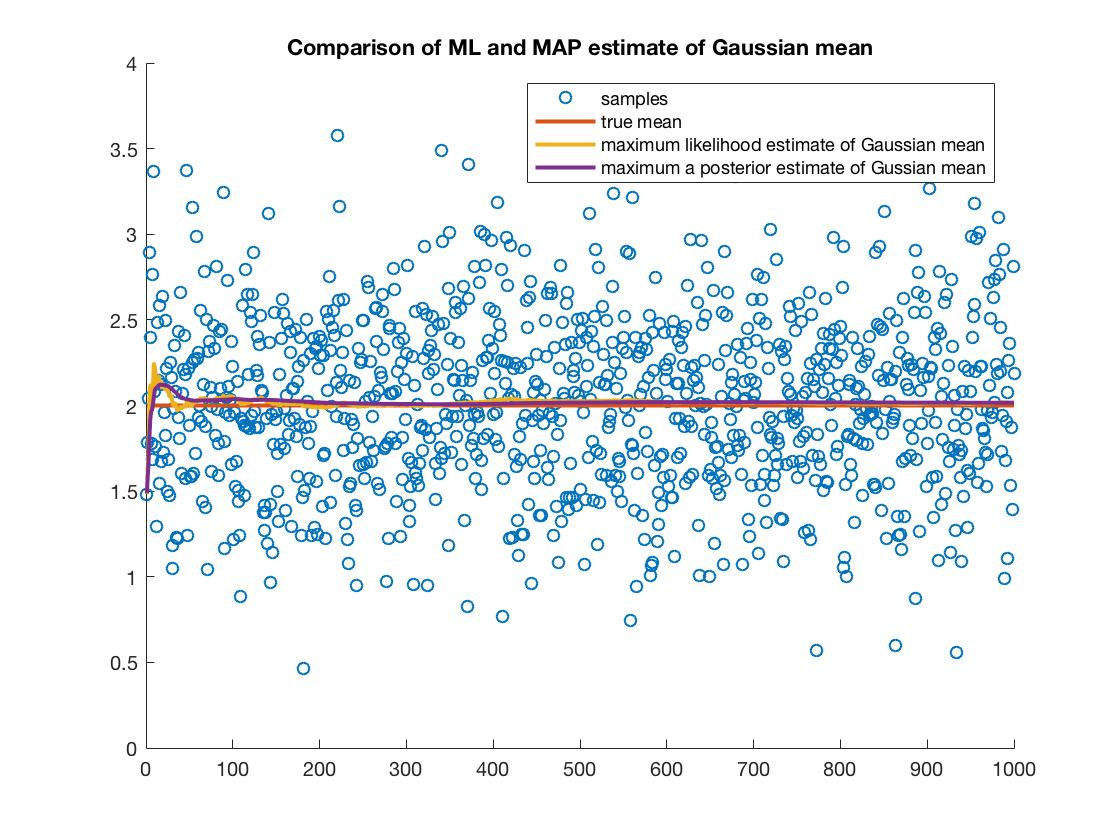
\includegraphics[width=4in]{exp7toConverge.jpg}
	\caption{When enough sample being drawn, even start with a big variance of the prior, the estimators would still converge to the true mean}
	\label{fig:side:b}
\end{figure}

\item In this case of comparison of varying \textbf{prior variance} from small to large, we can also look on the results when the prior of mean being  ``wrong" value, i.e. $\mu_0 =4$. Comparing the results of experiments 1 and 3. 
\begin{figure}[H]
	\centering
	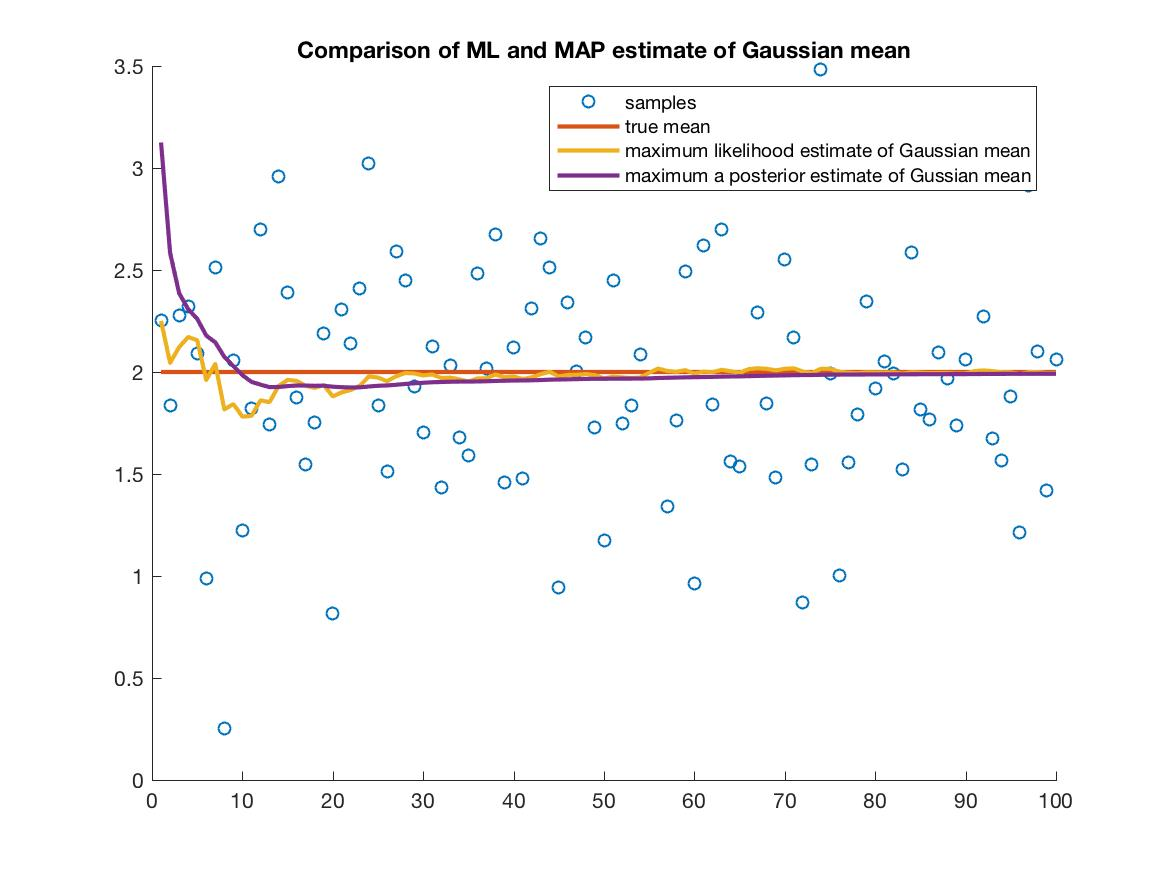
\includegraphics[width=3in]{100comparison1.jpg}
	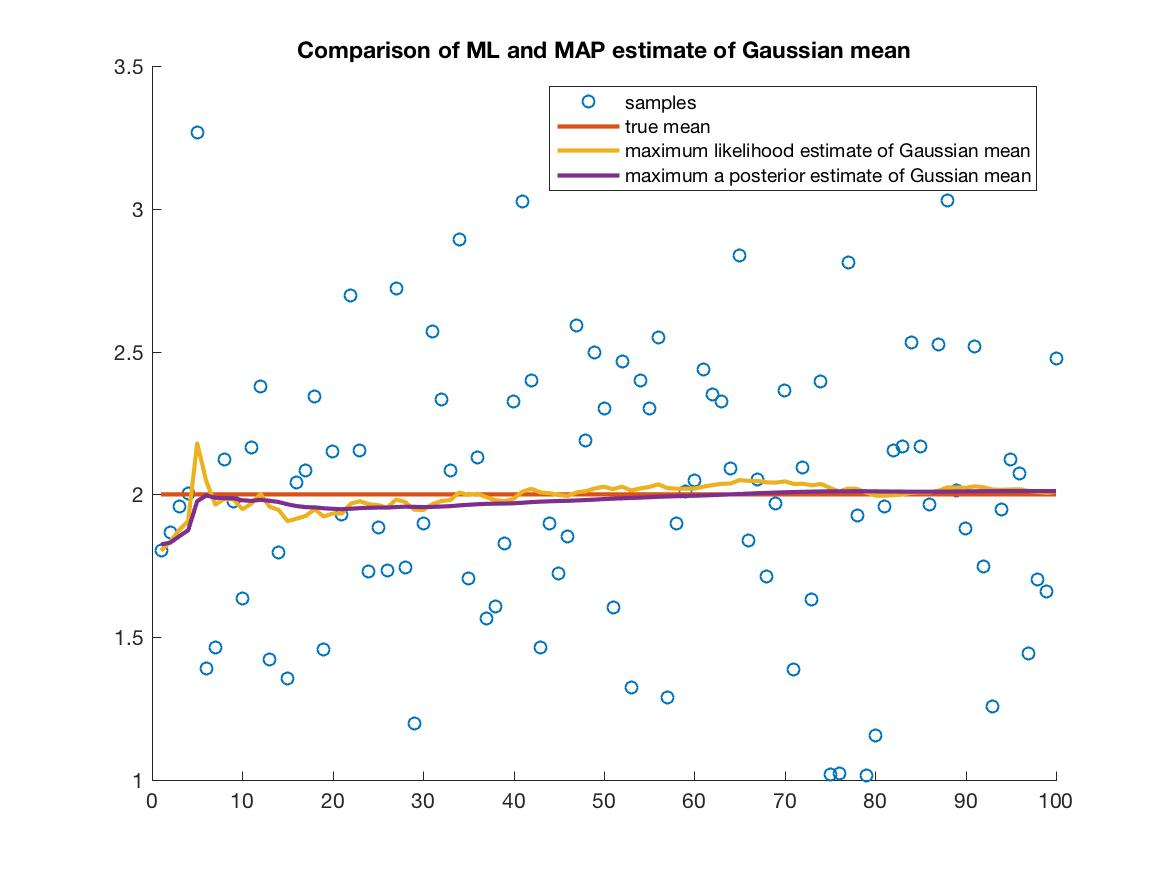
\includegraphics[width=3in]{100comparison3.jpg}
	\caption{left: comparison with small prior varianc(Exp1). right: comparison with large prior variance(Exp3).}
	\label{fig:side:b}
\end{figure}

\newpage
\item
Comparison of varying the \textbf{likelihood variance} from small to large by comparing the results of experiments 5 and 6, with $\mu_0 = 2$, $\sigma_0 = 0.5$ fixed.
\begin{figure}[H]
	\centering
	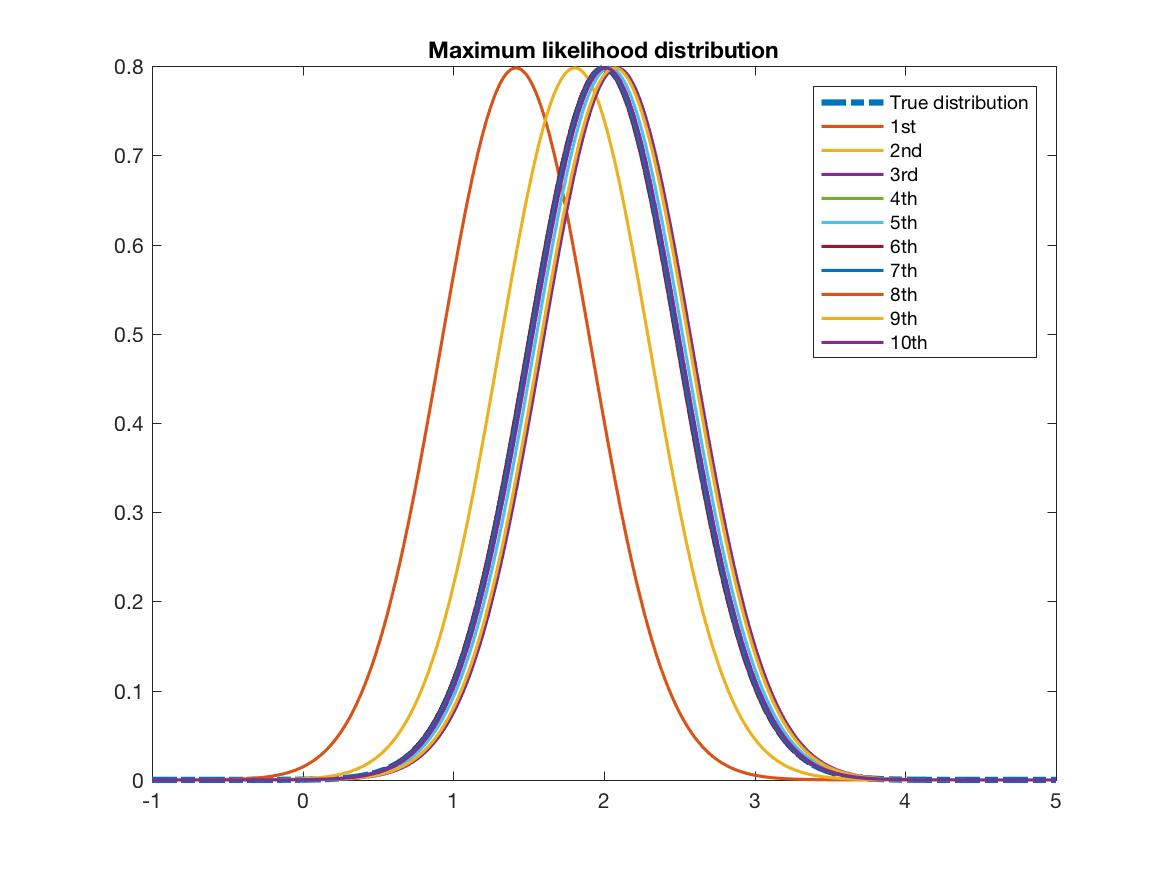
\includegraphics[width=3in]{ML5.jpg}
	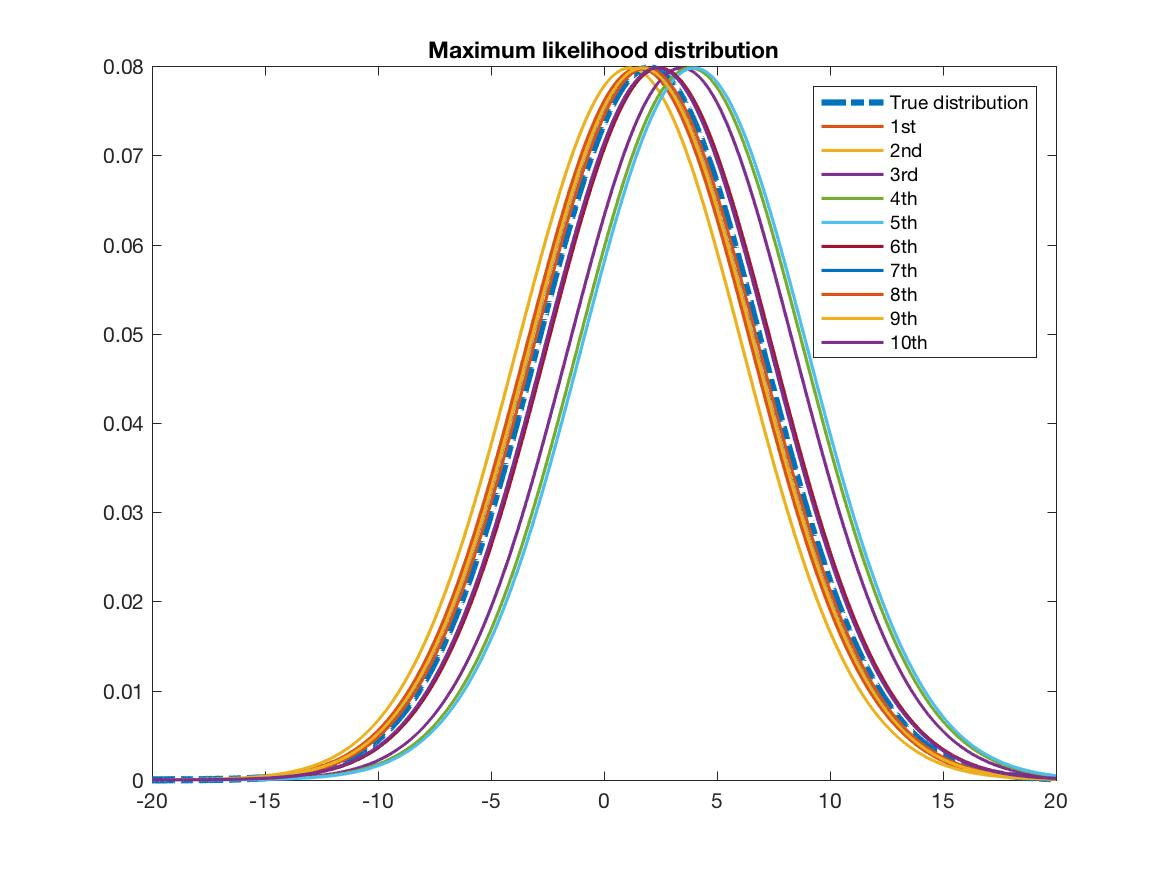
\includegraphics[width=3in]{ML6.jpg}
	\caption{left: ML with small likelihood variance(exp 5). right: ML with large likelihood variance(exp 6).}
	\label{q}
\end{figure}
\begin{figure}[H]
	\centering
	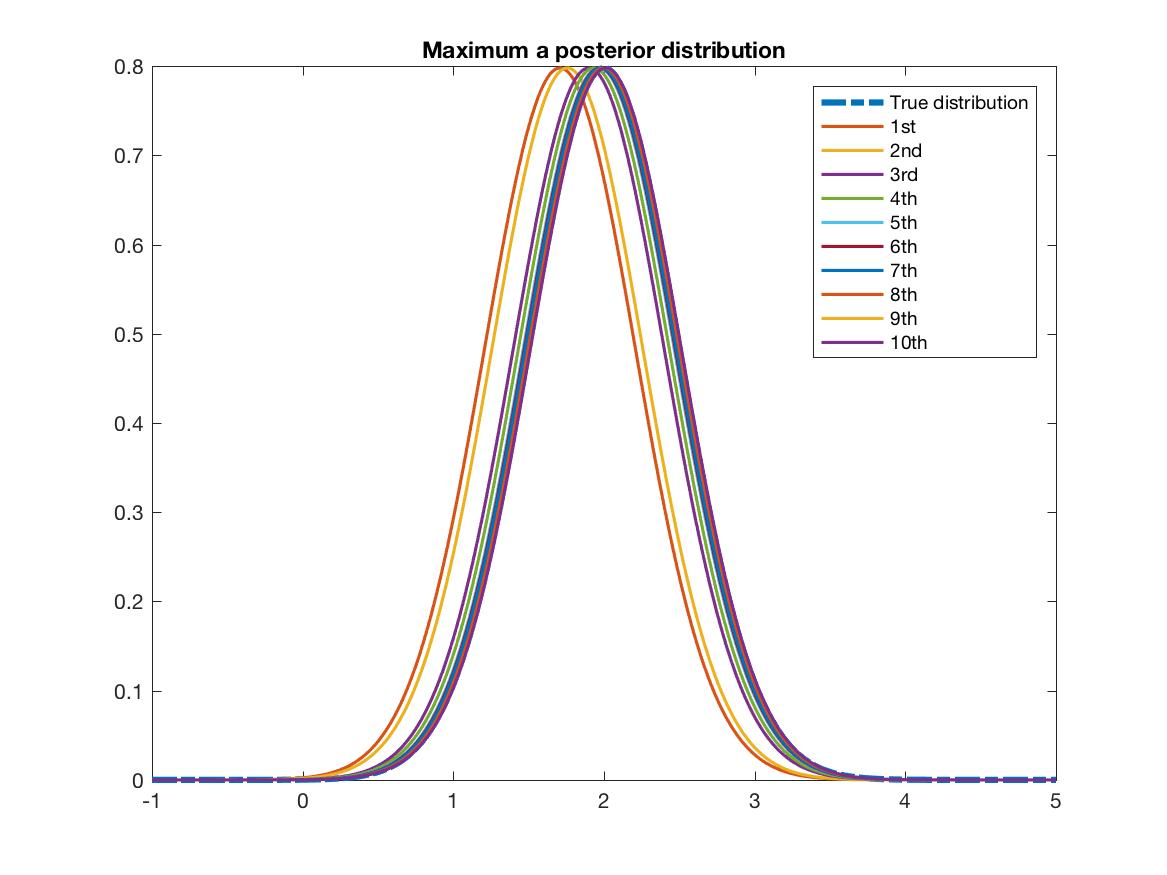
\includegraphics[width=3in]{MAP5.jpg}
	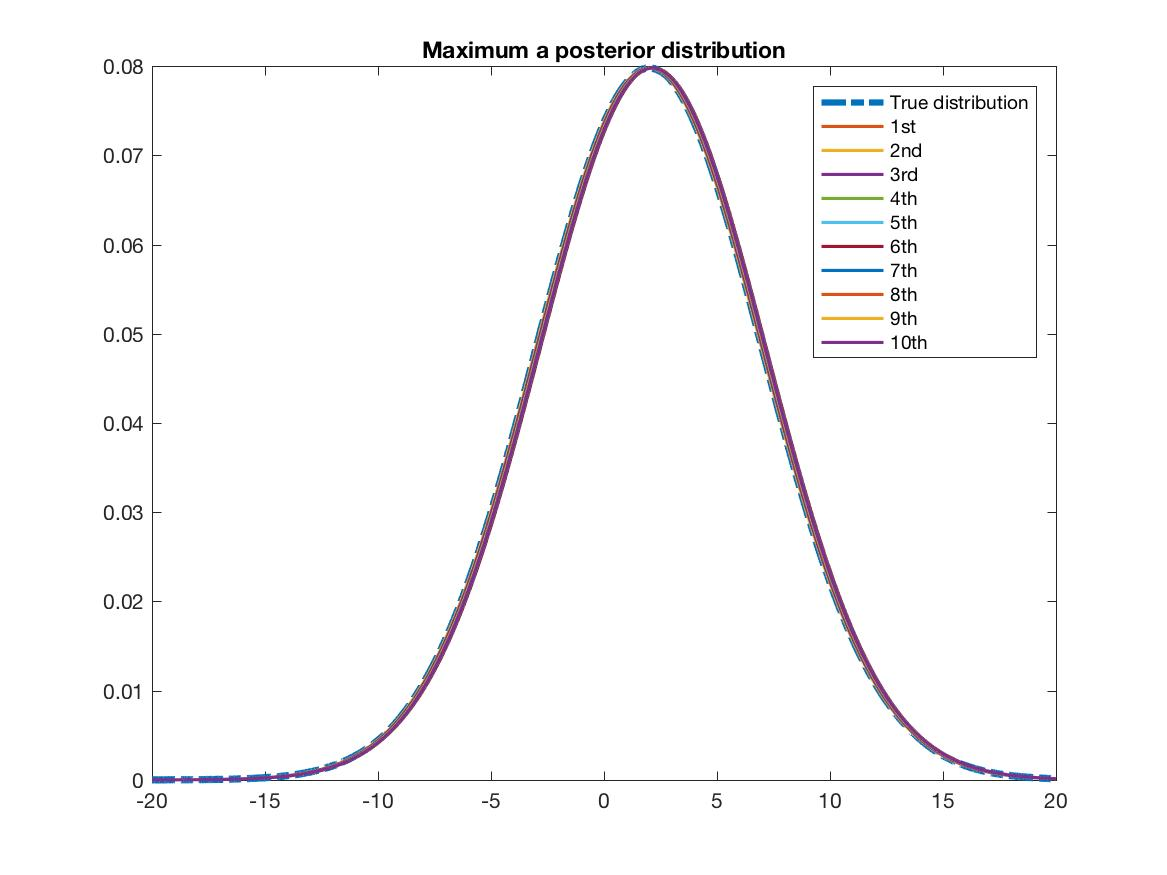
\includegraphics[width=3in]{MAP6.jpg}
	\caption{left: MAP with small likelihood variance(Exp 5). right: MAP with large likelihood variance(exp 6).}
	\label{fig:side:b}
\end{figure}
\begin{figure}[H]
	\centering
	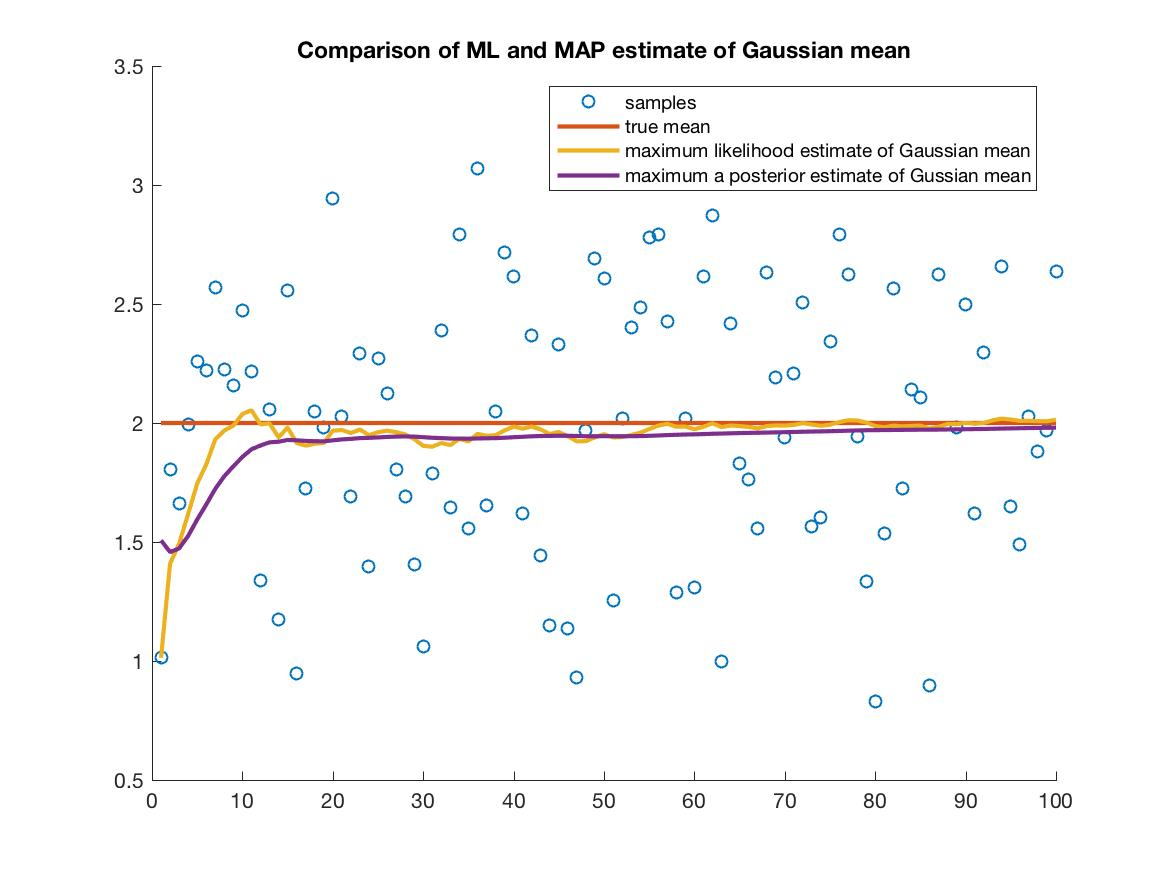
\includegraphics[width=3in]{100comparison5.jpg}
	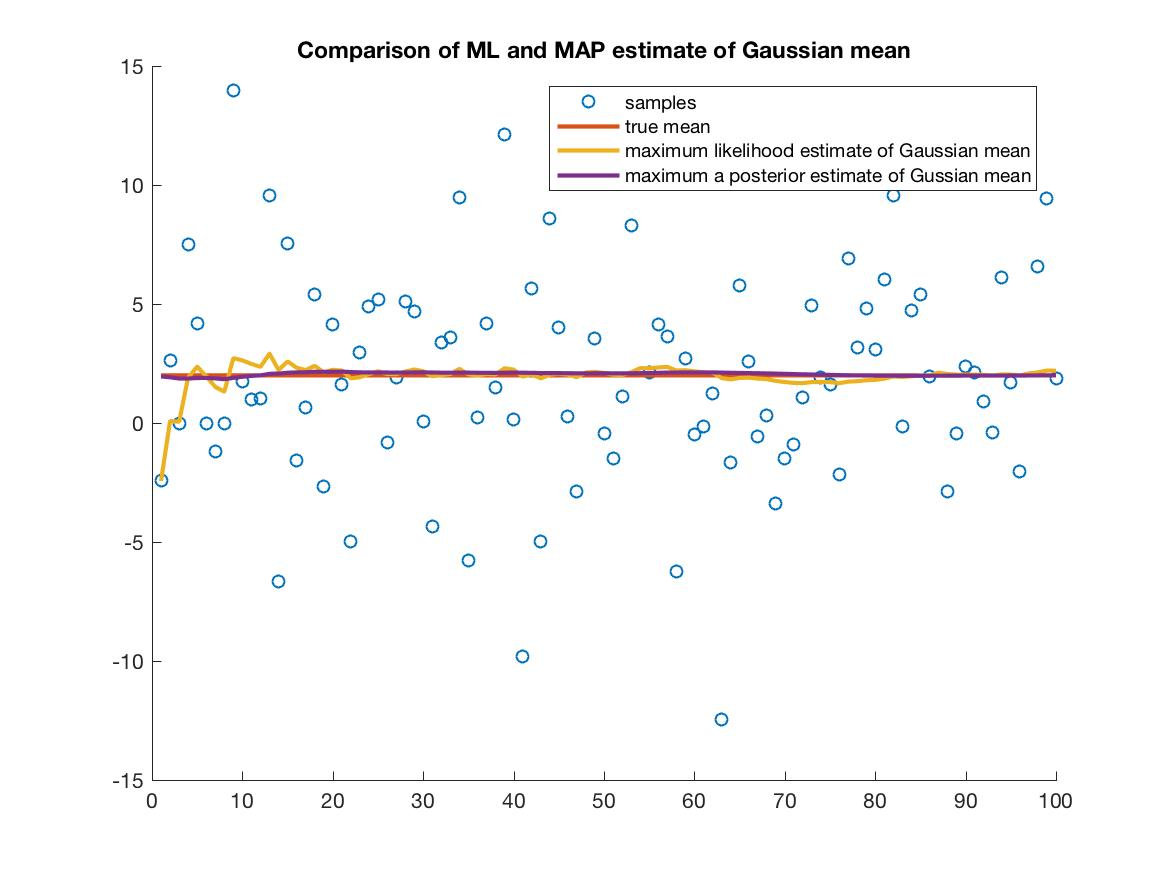
\includegraphics[width=3in]{100comparison6.jpg}
	\caption{left: comparison with small likelihood variance(Exp 5). right: with large likelihood variance(exp 6).}
	\label{fig:side:b}
\end{figure}
In this set of comparison I set the prior of mean to be the ``right" value, i.e. $\mu_0 = 2$. In this case, when the variance of the likelihood is comparatively large,  the MAP estimate of the mean converge much quickly compared to when the variance of the likelihood is small.
\item In this case of comparison of varying \textbf{likelihood variance} from small to large, we can also look on the results when the prior of mean being ``wrong" value, i.e. $\mu_0 =4$. Comparing the results of experiments 1 and 2.
\begin{figure}[H]
	\centering
	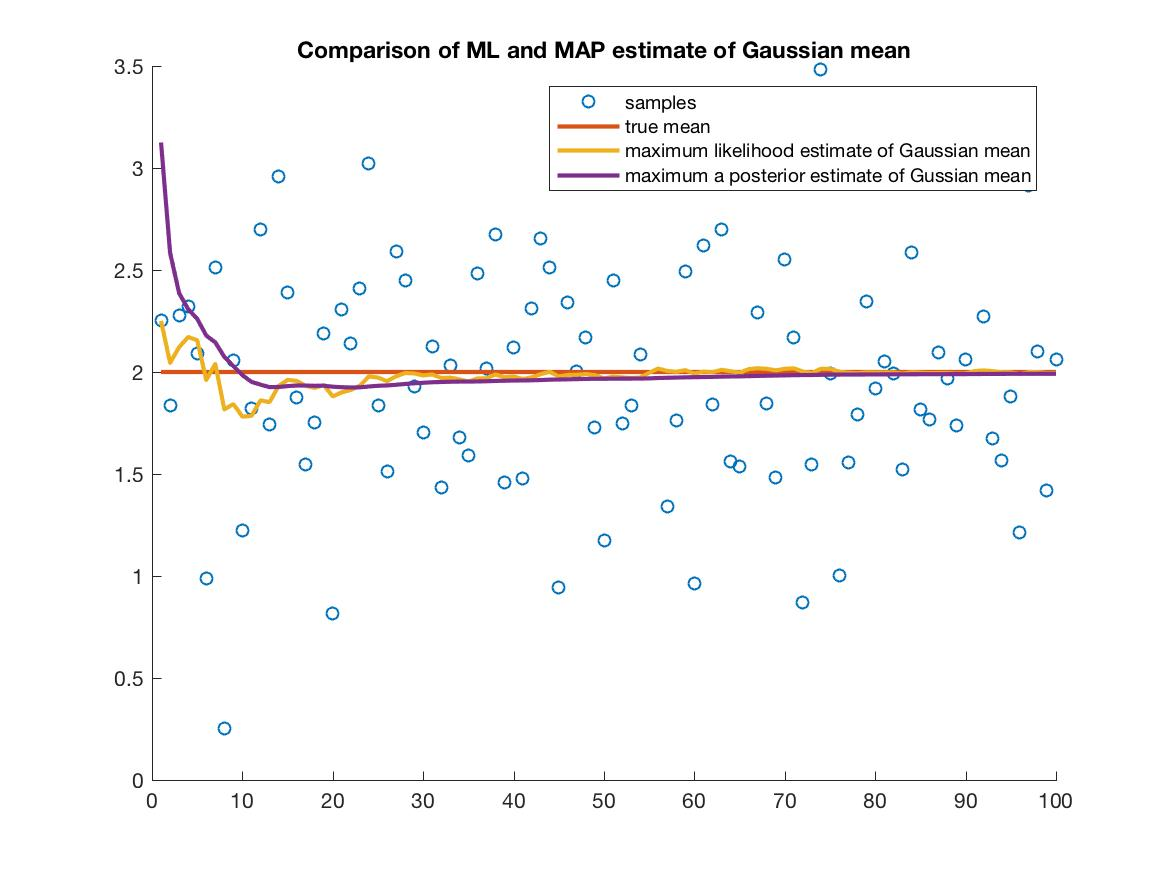
\includegraphics[width=3in]{100comparison1.jpg}
	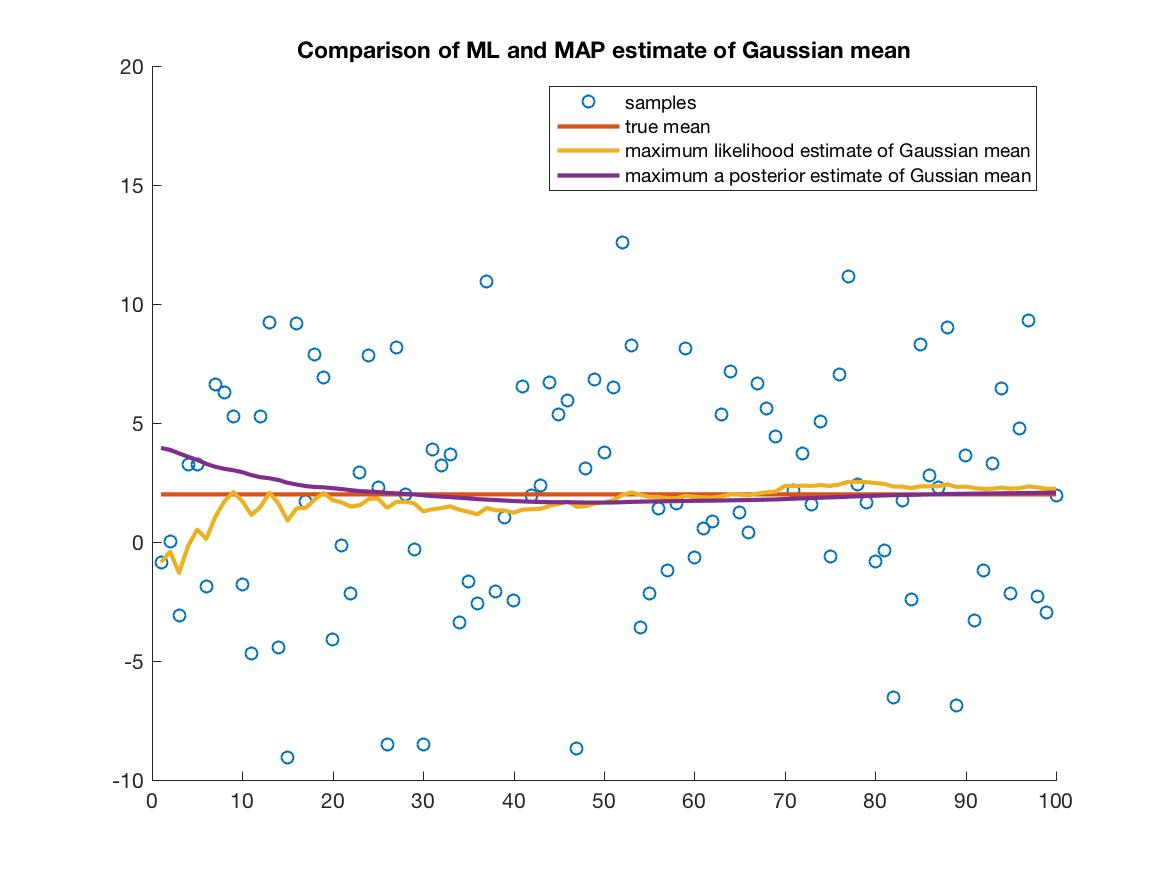
\includegraphics[width=3in]{100comparison2.jpg}
	\caption{left: comparison with small prior varianc(Exp1). right: comparison with large prior variance(Exp2).}
	\label{fig:side:b}
\end{figure}


I also included some discussion with regard to the posterior distribution of $\mu$.
\begin{figure}[H]
	\centering
	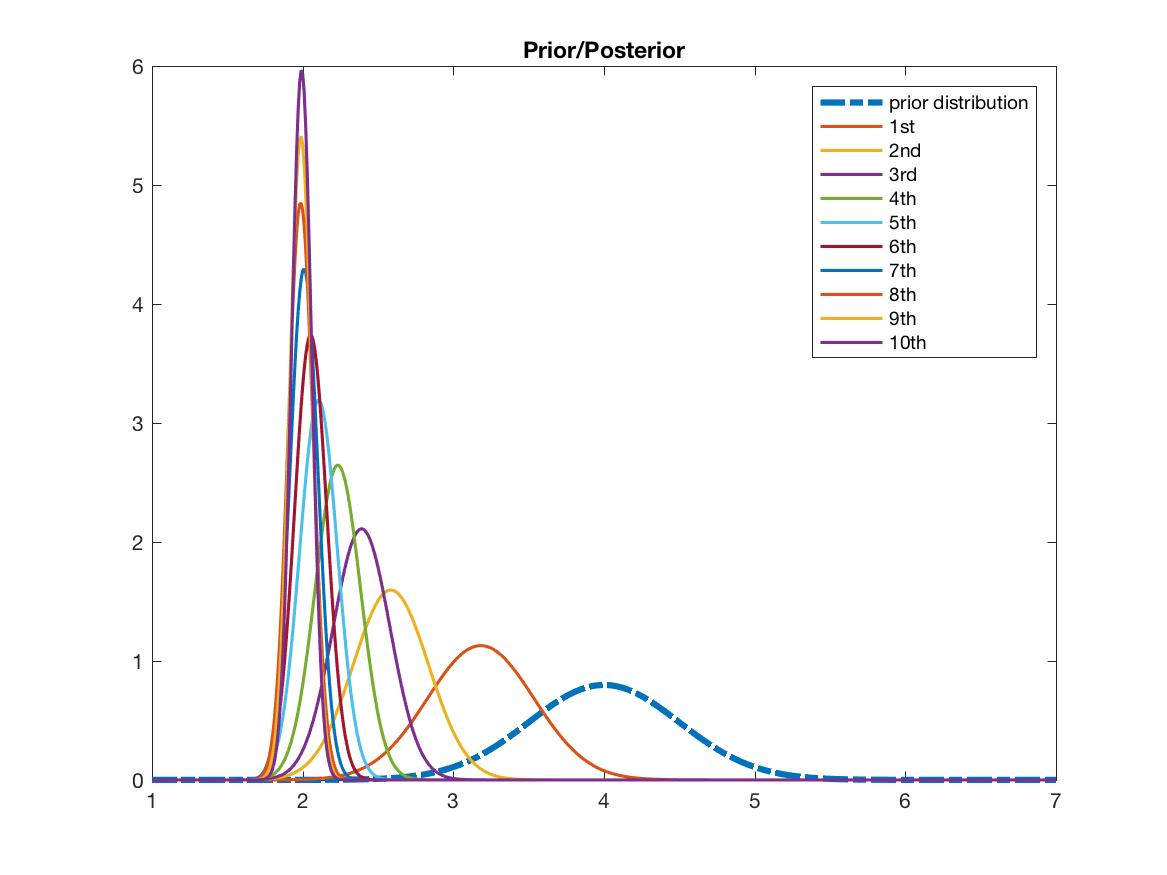
\includegraphics[width=3in]{posterior1.jpg}
	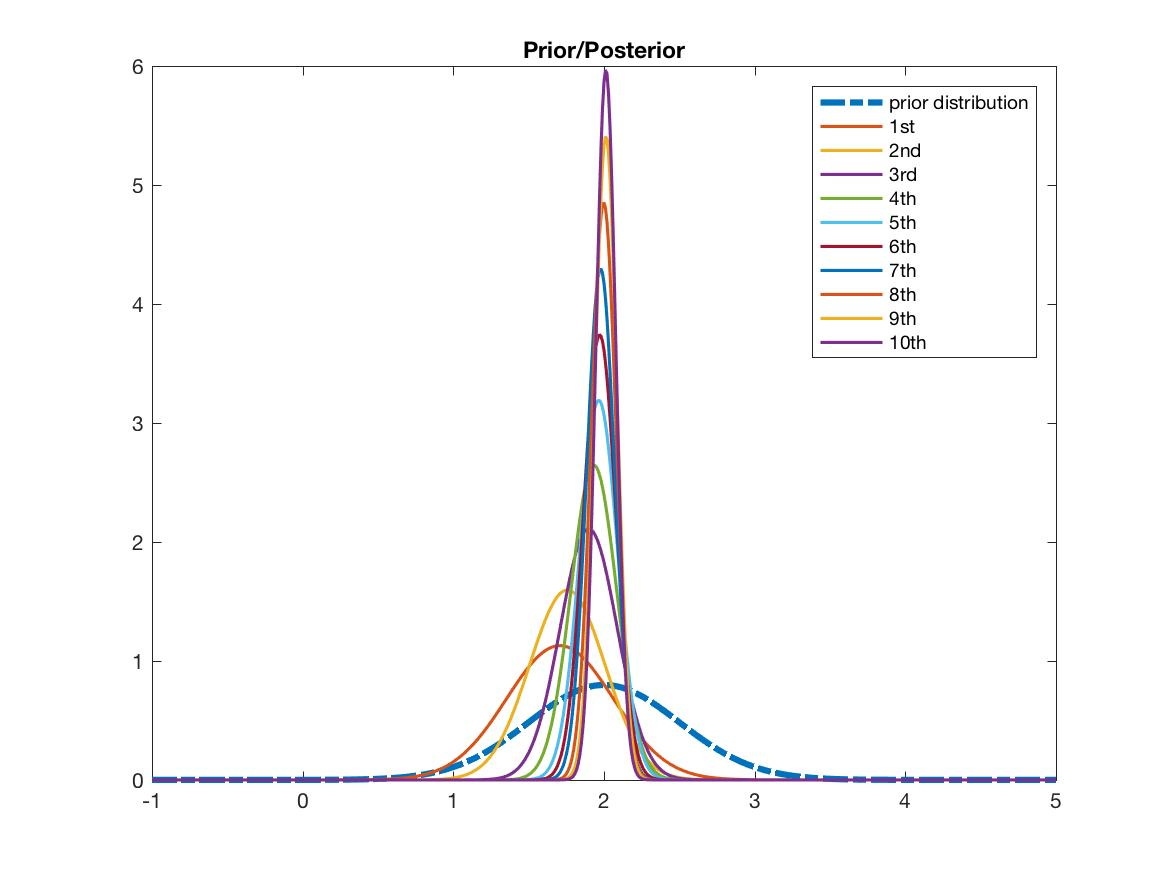
\includegraphics[width=3in]{posterior5.jpg}
	\caption{left: posterior distribution of $\mu$(Exp 1). right: posterior distribution of $\mu$(exp 5).}
	\label{fig:side:b}
\end{figure}

\begin{figure}[H]
	\centering
	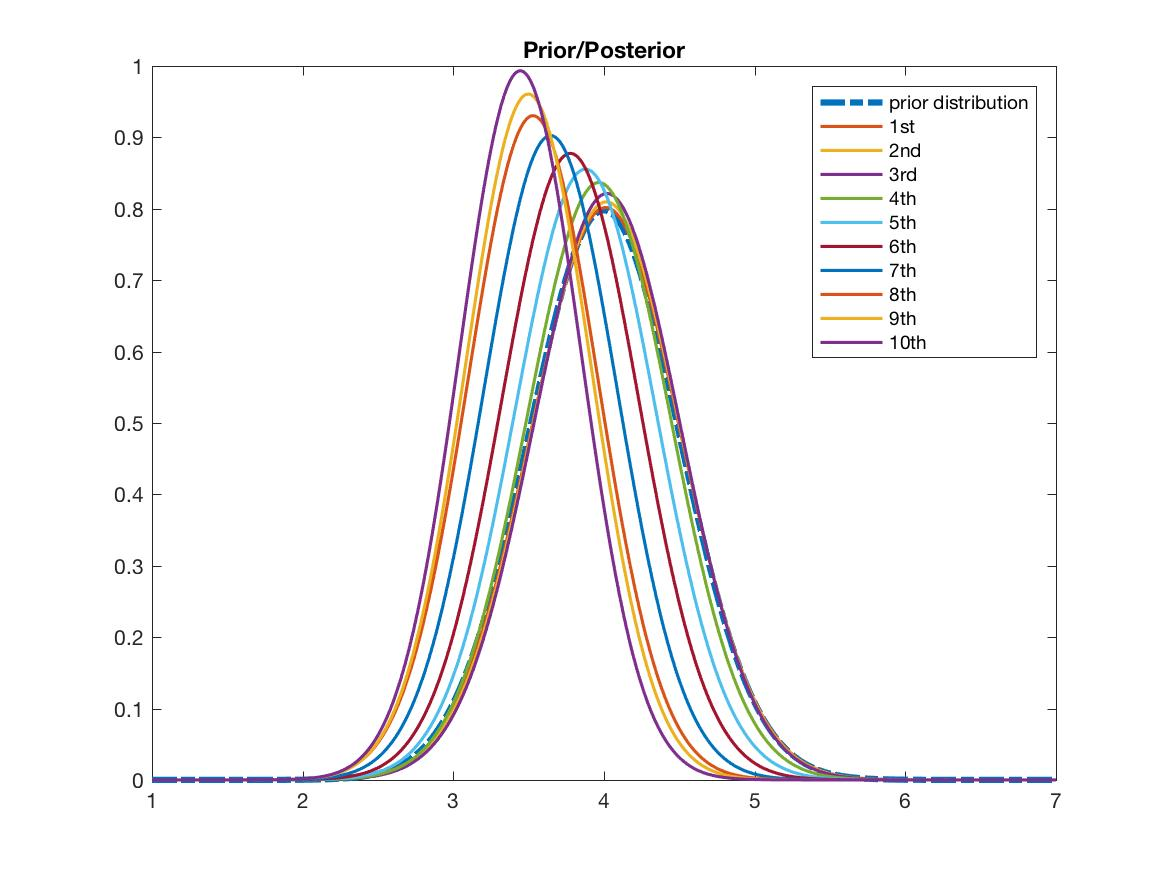
\includegraphics[width=3in]{posterior2.jpg}
	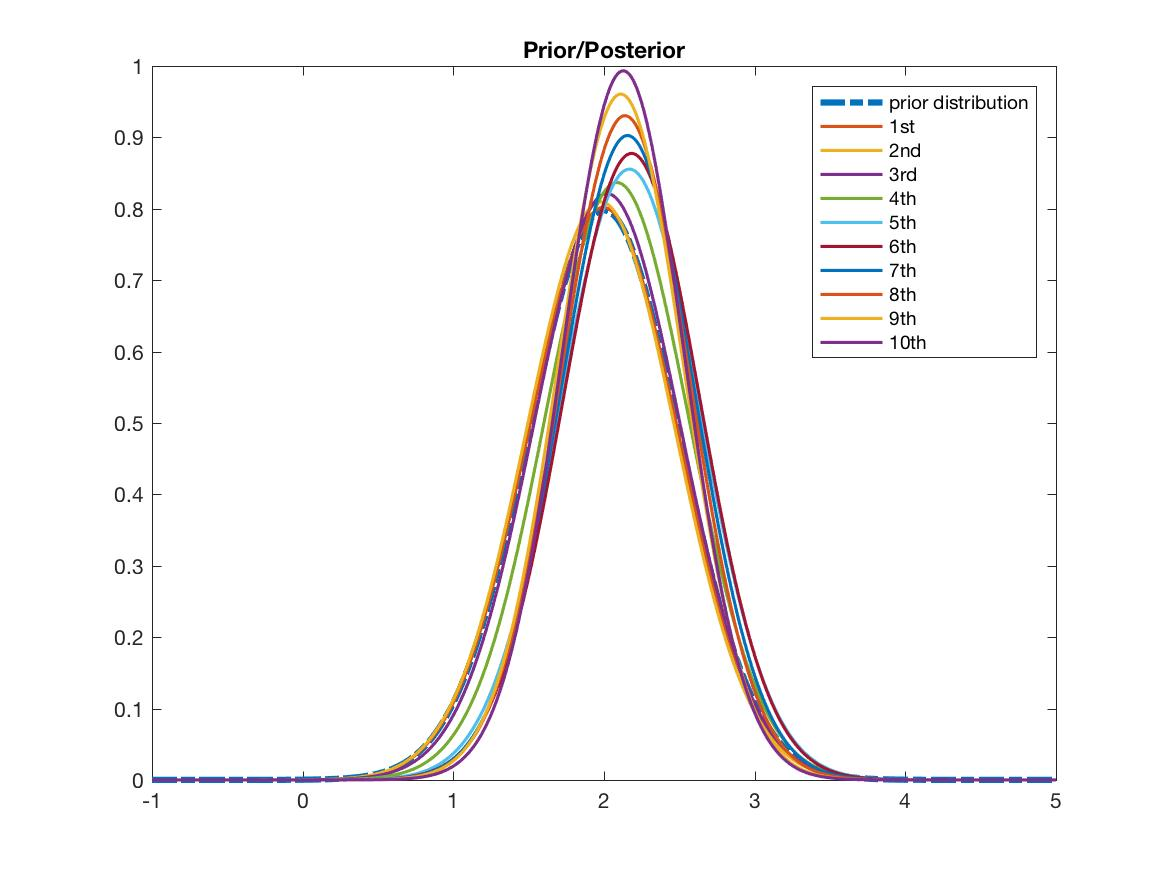
\includegraphics[width=3in]{posterior6.jpg}
	\caption{left: posterior distribution of $\mu$(Exp 2). right: posterior distribution of $\mu$(exp 6).}
	\label{fig:side:b}
\end{figure}

Based on this comparison, no matter the initialization of prior mean is initialized to a right value or wrong value, after enough iterations, the posterior distribution is center at the true mean, with the variance much smaller adding new sample. Which means that when enough sample is drawn, we become much confident with our posterior distribution of $\mu$. As is also seen from the formula: $\displaystyle\frac{1}{\sigma_N^2} = \displaystyle\frac{1}{\sigma_0^2} + \displaystyle\frac{N}{\sigma^2}$. As N becomes larger, the $\sigma_N$ becomes smaller with every new sample added, which means we are much confident with our estimate.\\

\newpage
To conclude, the experiment results justified what we learned from the formulas of posterior mean and posterior variance. Look at the formula of the posterior mean: 
$$\mu_N = \displaystyle\frac{\sigma^2}{N\sigma_0^2 + \sigma^2}\mu_0 + \displaystyle\frac{N\sigma_0^2}{N\sigma_0^2 + \sigma^2}\mu_{ML}$$
$$\displaystyle\frac{1}{\sigma_N^2} = \displaystyle\frac{1}{\sigma_0^2} + \displaystyle\frac{N}{\sigma^2}$$
we learned that the posterior mean is a weighted average of the prior mean and maximum likelihood estimate of the mean. And the reciprocal of the posterior variance is also a weighted combination of the reciprocal of the prior variance and the reciprocal of the likelihood variance. Thus, several point are stated here:
\begin{enumerate}
\item When more samples are generated from the distribution we are to estimate the mean from, the weight for the maximum likelihood estimator becomes larger, thus when getting much sample, the maximum a posterior solution would converge to the maximum likelihood solution. And the posterior variance becomes smaller with samples added, which means we become much confident with the knowledge regarding the mean we are to estimate.
\item When the likelihood variance is small, much weight is put on the ML solution, thus the MAP solution get much influence from the data rather than the prior. So in this case, even a wrong prior on the mean is assumed, when the variance of likelihood is small, the MAP is able to converge to ML solution quickly. While conversely, when the variance of likelihood is large, and the assumption on the prior is wrong, it would take longer time for MAP to converge.
\item When the prior variance is small, much weight is put on the prior, which means it is essential to get a prior mean close to the true mean, otherwise it may takes long for MAP solution to converge.
\end{enumerate}

\newpage
Code that used in this report:
\begin{lstlisting}
clear; close all; clc
exp = 3;
%% true mean and standard deviation of the distribution
num_x = -1:0.01:5;%-20:0.01:20;%
mu = 2;
sigma = 0.5; %5;%standard deviation 
true_dist = normpdf(num_x, mu, sigma);
figure(1), plot(num_x, true_dist, '-.', 'Linewidth', 3), ...
hold on, saveas(gcf, ['trueDist' num2str(exp) '.jpg'])
figure(2), plot(num_x, true_dist, '-.', 'Linewidth', 3), ...
hold on, saveas(gcf, ['trueDist' num2str(exp) '.jpg'])
%% initialize the prior of the Gaussian mean
num_mu = -1:0.01:5;
mu_0 = 2;%4;%
sigma_0 = 0.5; %standard deviation5; %
prior = normpdf(num_mu, mu_0, sigma_0);
figure(3), plot(num_mu, prior, '-.','Linewidth', 3), ...
hold on, saveas(gcf, ['prior' num2str(exp) '.jpg'])
%% initialize the posterior of the Gaussian mean
mu_N = mu_0;
sigma_N = sigma_0;
posterior = normpdf(num_mu, mu_N, sigma_N);
%%
num_Sample = 100;
sample = [];
true_prob = [];
ML_prob = [];
MAP_prob = [];
mu_ML = [];
mu_MAP = [];
for iter = 1:num_Sample
    mu_0 = mu_N; %update the prior mean with the posterior mean from the previous draw
    sigma_0 = sigma_N; %update the prior variance(standard deviation) with the posterior variance from the previous draw
    sample = [sample normrnd(mu,sigma)]; %get a sample from the true distribution
    N = length(sample);
    mu_ML = [mu_ML mean(sample)]; %ML solution for the Gaussian mean
    ML = normpdf(num_x, mu_ML(N), sigma);
    figure(1), plot(num_x, ML, 'Linewidth', 1.5), hold on 
    mu_N = mu_0*sigma^2/(N*sigma_0^2 + sigma^2) ...
    + mu_ML(N)*N*sigma_0^2/(N*sigma_0^2 + sigma^2); %MAP solution for the Gaussian mean
    sigma_N = sqrt(1/(1/sigma_0^2+N/sigma^2)); %standard deviation of the posterior
    MAP = normpdf(num_x, mu_N, sigma);
    figure(2), plot(num_x, MAP, 'Linewidth', 1.5), hold on
    mu_MAP = [mu_MAP mu_N];
    posterior_ = normpdf(num_mu, mu_N, sigma_N);
    figure(3), plot(num_mu, posterior_, 'Linewidth', 1.5), hold  on 
    display(['random data point from Gaussian is ' num2str(sample(N))])
    display(['Maximum likelihood solution of mean is ' num2str( mu_ML)])
    display(['Maximum a posterior solution of mean is ' num2str(mu_N)])
    true_prob = [true_prob cdf('Normal',sample(N),mu,sigma)];
    ML_prob = [ML_prob cdf('Normal',sample(N),mu_ML(N),sigma)];
    MAP_prob = [MAP_prob cdf('Normal',sample(N),mu_N,sigma)];
    display(['True probablity of drawing ' num2str(sample(N)) ' ...
    from Gaussian is ' num2str(cdf('Normal',sample(N),mu,sigma))])
    display(['ML probablity of drawing ' num2str(sample(N)) ' ...
    from Gaussian is ' num2str(cdf('Normal',sample(N),mu_ML(N),sigma))])
    display(['MAP probability of drawing ' num2str(sample(N)) ' ...
    from Gaussian is ' num2str(cdf('Normal',sample(N),mu_N,sigma))]) 
end
figure(1), title('Maximum likelihood distribution'), ...
saveas(gcf, ['ML' num2str(exp) '.jpg'])
figure(2), title('Maximum a posterior distribution'), ...
saveas(gcf, ['MAP' num2str(exp) '.jpg'])
figure(3), title('Prior/Posterior'), ...
saveas(gcf, ['posterior' num2str(exp) '.jpg'])
tosave = [sample;true_prob; ML_prob; MAP_prob; mu_ML; mu_MAP];
figure(4), scatter(1:N, sample), hold on, plot(mu*ones(1,N), 'Linewidth', 2), hold on, plot(mu_ML, 'Linewidth', 2),...
 hold on, plot(mu_MAP, 'Linewidth', 2)
title('Comparison of ML and MAP estimate of Gaussian mean')
saveas(gcf, [num2str(num_Sample) 'comparison' num2str(exp) '.jpg'])
\end{lstlisting}

\end{itemize}
\end{spacing}
\end{document}